%----------------------------------------------------------------------------------------
%	1. DOCUMENT CLASS AND THEME
%----------------------------------------------------------------------------------------
\PassOptionsToPackage{table}{xcolor}
\documentclass[aspectratio=169,xcolor=dvipsnames,10pt]{beamer}

% THEME SETUP
\usetheme{SimplePlusAIC}
\useinnertheme[showtitle=false]{tcolorbox}
\setbeamerfont{section in toc}{size=\small}
\setbeamerfont{block title}{size=\small}

% --- FIX TITLE BACKGROUND ---
% Force the title box to have no background color (transparent)
% so the Beige canvas shows through.
%\setbeamercolor{title}{bg=} 
%\setbeamercolor{frametitle}{bg=}
%\setbeamercolor{title}{bg=OffWhite}
%\setbeamercolor{frametitle}{bg=OffWhite}

% COLOR DEFINITIONS
\definecolor{OffWhite}{RGB}{255, 254, 245}
\definecolor{Beige}{RGB}{245, 245, 220}
\setbeamercolor{background canvas}{bg=OffWhite}

% 2. Force ALL title page elements to have a transparent background
%\setbeamercolor{title}{bg=OffWhite}         % Clear background for Title
%\setbeamercolor{subtitle}{bg=OffWhite}      % Clear background for Subtitle
%\setbeamercolor{author}{bg=OffWhite}        % Clear background for Author
%\setbeamercolor{institute}{bg=OffWhite}     % Clear background for Institute
%\setbeamercolor{date}{bg=OffWhite}          % Clear background for Date

%----------------------------------------------------------------------------------------
%	2. PACKAGES
%----------------------------------------------------------------------------------------

% --- MATH & FONTS ---
\usepackage{amsmath}
\usepackage{amssymb}
\usepackage{amsfonts}
\usepackage{bm}           % Bold math symbols
\usepackage{relsize}
\usefonttheme[onlymath]{serif}

% --- GRAPHICS, TIKZ & PLOTS ---
\usepackage{graphicx}
\usepackage{subcaption}
\usepackage{svg}
\usepackage{animate}
\usepackage{wrapfig}
\usepackage{tikz}
\usepackage{pgfplots}     
\pgfplotsset{compat=1.18} 
\usetikzlibrary{shapes,arrows.meta,positioning,fit,calc,backgrounds,intersections}

% --- TABLES & UTILITIES ---
\usepackage{booktabs}
\usepackage{makecell}
\usepackage{multirow}
\usepackage{hhline}
\usepackage{ragged2e}
\usepackage{verbatim}
\usepackage{caption}
\usepackage{appendixnumberbeamer}

% --- CUSTOM BOXES ---
\usepackage{tcolorbox}
\tcbuselibrary{skins, breakable}

%----------------------------------------------------------------------------------------
%	3. ALGORITHMS (STRICT LOAD ORDER)
%----------------------------------------------------------------------------------------
\usepackage{float}

% 1. Standard Algorithm (Legacy support)
\usepackage{algorithm} 
\usepackage{algpseudocode}
% Fix for \ALG@currentblock@0 error in Beamer
\algblockdefx{While}{EndWhile}{\textbf{while} }{}

% 2. Algorithm2e (Modern support)
% 'algo2e' option prevents clash with the 'algorithm' package above.
% You must use \begin{algorithm2e} ... \end{algorithm2e} for this style.
\usepackage[ruled,vlined,algo2e]{algorithm2e} 

% --- REFERENCES (MUST BE LAST) ---
\usepackage{hyperref}
\usepackage{cleveref}

%----------------------------------------------------------------------------------------
%	4. CONFIGURATION & COMMANDS
%----------------------------------------------------------------------------------------

% --- SAFE CONFIGURATION FOR ALGORITHMS ---
\AtBeginDocument{
    \crefname{algocf}{algorithm}{algorithms} 
    \crefname{algorithm}{algorithm}{algorithms}
}

% --- BOX DEFINITIONS ---
\newtcolorbox[auto counter, number within=section]{roundedshadowbox}[2][]{
    colback=white,
    colframe=black,
    boxrule=0.5pt,
    arc=5mm,
    shadow=true,
    width=\linewidth,
    title=#2,
    #1
}

% --- MATH MACROS ---
\newcommand*{\defeq}{\stackrel{\text{def}}{=}}
\newcommand{\grad}{\nabla}
\newcommand{\lap}{\Delta}
\newcommand{\weaklyto}{\rightharpoonup}
\newcommand{\weakstar}{\stackrel{*}\rightharpoonup}
\newcommand{\cts}{\hookrightarrow}
\newcommand{\ctsDense}{\xhookrightarrow{d}}
\newcommand{\ctsCompact}{\xhookrightarrow{c}}

% Sets
\newcommand{\R}{\mathbb{R}}
\newcommand{\bR}{\mathbb{R}}
\newcommand{\C}{\mathbb{C}}
\newcommand{\E}{\mathbb{E}}
\newcommand{\bE}{\mathbb{E}}
\newcommand{\pP}{\mathbb{P}}
\newcommand{\bP}{\mathbb{P}}
\newcommand{\ER}{\overline{\mathbb{R}}}

% Calligraphic
\newcommand{\fF}{\mathfrak{F}}
\newcommand{\cP}{\mathcal{P}}
\newcommand{\cR}{\mathcal{R}}
\newcommand{\cJ}{\mathcal{J}}
\newcommand{\cG}{\mathcal{G}}
\newcommand{\cU}{\mathcal{U}}
\newcommand{\cX}{\mathcal{X}}
\newcommand{\cY}{\mathcal{Y}}
\newcommand{\cZ}{\mathcal{Z}}
\newcommand{\cF}{\mathcal{F}}

% Operators
\newcommand{\CVaR}{\textup{CVaR}}
\newcommand{\D}{\textup{ d}}
\newcommand{\dd}{\mathrm{d}}
\newcommand{\fa}{\text{for all }}
\DeclareMathOperator*{\essinf}{\vphantom{p}ess\,inf}
\DeclareMathOperator{\sigmoid}{expit}

% Specifics
\newcommand{\Xad}{\mathcal{X}_{\text{\textup{ad}}}}
\newcommand{\Zad}{\mathcal{Z}_{\text{\textup{ad}}}}
\newcommand{\Lp}[1]{L^{#1}(\Omega,\mathcal{F},\mathbb{P})}
\newcommand{\riskenv}{\mathfrak{A}}
\newcommand{\fP}{\mathfrak{P}}
\newcommand{\risk}{\mathcal{R}}
\newcommand{\bbe}{\mathbb{E}}
\newcommand{\bbp}{\mathbb{P}}
\newcommand{\Pae}{\mathbb{P}\text{-a.e.}}

\newtheorem{proposition}{Proposition}
\newcommand{\slidefootnote}[1]{\vspace*{\fill}{\footnotesize #1}}

% --- BACKGROUND LOGO ---
\setbeamertemplate{background}{\tikz[overlay,remember picture]\node[opacity=0.05,anchor=south west]
at (current page.south west)
{
\includegraphics[width=5cm,keepaspectratio]{logos/Simula_logo.png}};}

%----------------------------------------------------------------------------------------
%	5. TITLE INFO
%----------------------------------------------------------------------------------------
\title[LaVa]{The Latent Variable Proximal Point Method\\  A structure‐preserving approach to
constrained variational problems.}
\author{\small{\bf Thomas M. Surowiec}}
\institute[T.M. Surowiec]{Department of Numerical Analysis and Scientific Computing \newline Simula Research Laboratory \newline Oslo, Norway}
\date{\hfil Oslo, 26 January 2026}

%----------------------------------------------------------------------------------------
%	FIX: CLEAN TITLE PAGE (No Shadows, Transparent Backgrounds)
%----------------------------------------------------------------------------------------

% 1. Force the title page to use the default layout.
%    This strips away the "fancy" boxes/shadows that the theme applies,
%    leaving just the text and your logo.
\setbeamertemplate{title page}[default]

% 2. Ensure all title elements are strictly transparent.
%    (The 'bg=' sets the background to empty/none).
\setbeamercolor{title}{bg=}
\setbeamercolor{subtitle}{bg=}
\setbeamercolor{author}{bg=}
\setbeamercolor{institute}{bg=}
\setbeamercolor{date}{bg=}

% 3. Optional: Restore bold/size if the [default] template resets them too much.
\setbeamerfont{title}{size=\Large, series=\bfseries}
\setbeamerfont{author}{size=\large, series=\bfseries}

\begin{document}

\begin{frame}[plain]
    \titlepage
\end{frame}

\begin{frame}[plain]
\centering
%[trim={left bottom right top},clip]
    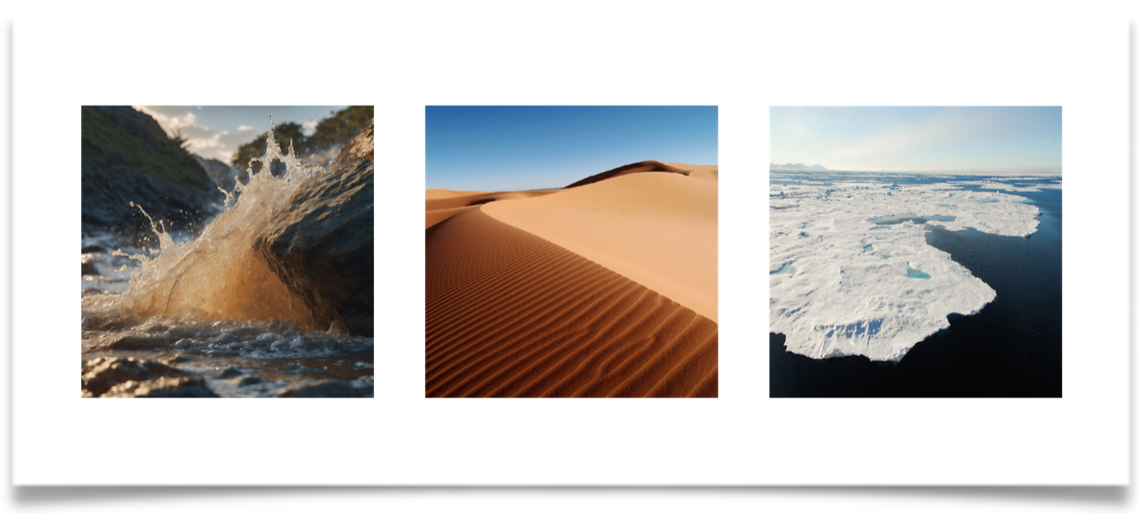
\includegraphics[width=0.7\linewidth,trim={0 1cm 0 0},clip]{figures/water-sand-ice.png}\bigskip
    
    \visible<2->{\centering The key modeling assumption requires the solutions to satisfy \textit{\alert{inequality constraints}}.} \bigskip
    
    \visible<3->{\centering Why is this challenging?}
    
\end{frame}

\begin{frame}{What are partial differential equations?}

    % 1. DYNAMIC HEADER
    \centering
    \textcolor{NavyBlue}{\small \textbf{
        \only<1>{Step 1: Newton's Law (Static Equilibrium)}%
        \only<2>{Step 2: The Discrete Stencil}%
        \only<3>{Step 3: The Continuous Limit ($h \to 0$)}%
        \only<4->{Step 4: Generalizing to Poisson}%
    }}

    \vspace{0.2cm}

%Here is the corrected logic:
%Tension Forces ($N$): Depend on the slope ($\approx \frac{\Delta u}{h}$).
%External Load ($N$): Depends on density times length ($f \cdot h$).
%The Division: When we divide the whole equation by $h$ to get back to a density equation, the tension term (which already had an $h$ in the denominator from the slope) gets another $h$, creating the $h^2$.

    % 2. STEP 1: PHYSICS (New)
    \only<1-3>{
        \begin{block}{Force Balance on an Elastic String}
            \begin{columns}
                \column{0.6\textwidth}
                \small
                A point $x$ is pulled by tension $T$ from neighbors $x{\pm}h$.\\ The forces should be in equilibrium with external load $f$:
                \begin{equation*}
                  \underbrace{\frac{T}{h}(u_{x-h} - u_x)}_{\text{Left Pull}} + 
                  \underbrace{\frac{T}{h}(u_{x+h} - u_x)}_{\text{Right Pull}} + f(x)\cdot h = 0
                \end{equation*}
                
                \column{0.35\textwidth}
                \centering
                % TikZ Diagram of String Segment
                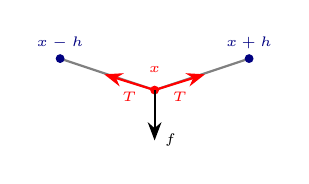
\begin{tikzpicture}[scale=0.8]
                    % String
                    \draw[thick, gray] (-1.5,0.5) -- (0,0) -- (1.5,0.5);
                    % Points
                    \fill[NavyBlue] (-1.5,0.5) circle (2pt) node[above] {\tiny $x-h$};
                    \fill[Red] (0,0) circle (2pt) node[above=3pt] {\tiny $x$};
                    \fill[NavyBlue] (1.5,0.5) circle (2pt) node[above] {\tiny $x+h$};
                    % Forces
                    \draw[-{Stealth}, Red, thick] (0,0) -- (-0.8, 0.25) node[midway, below] {\tiny $T$};
                    \draw[-{Stealth}, Red, thick] (0,0) -- (0.8, 0.25) node[midway, below] {\tiny $T$};
                    \draw[-{Stealth}, black, thick] (0,0) -- (0,-0.8) node[right] {\tiny $f$};
                \end{tikzpicture}
            \end{columns}
        \end{block}
    }

    % Arrow 1
%    \visible<2->{\begin{center}\vspace{-0.2cm}\tikz{\draw[-{Stealth}, gray] (0,0) -- (0,-0.2);}\vspace{-0.2cm}\end{center}}

    % 3. STEP 2: FINITE DIFFERENCES
    \only<2>{
        \begin{block}{The Discrete Stencil}
            Rearranging the terms and scaling by length $h^2$:
            \begin{equation*}
                 \frac{-u(x-h) + 2u(x) - u(x+h)}{h^2} \approx f(x)
            \end{equation*}
        \end{block}
    }

    % Arrow 2
%    \visible<3->{\begin{center}\vspace{-0.2cm}\tikz{\draw[-{Stealth}, gray] (0,0) -- (0,-0.2);}\vspace{-0.2cm}\end{center}}

    % 4. STEP 3: DERIVATIVES
    \only<3>{
        \begin{block}{Continuous Limit: Zoom out, nature is often continuous!}
            As $h \to 0$, the difference quotient becomes the negative curvature:
            \vspace{-0.2cm}
            \begin{equation*}
                -\frac{\partial^2 u}{\partial x^2} = f(x)
            \end{equation*}
            This is called an \textit{\alert{ordinary differential equation}} or simply \textit{\alert{ODE}}.
        \end{block}
    }

%We start with a discrete set of points connected by forces. But nature is often continuous. If we let the distance between these points, $h$, shrink to zero, this discrete difference quotient transforms into the second derivative. This bridges the gap between a simple system of springs and the continuous Laplace operator.

% 3. 2D EXTENSION (Visible 3+) - THE NEW BRIDGE
    \only<4->{
        \begin{block}{2D: Forces on a Membrane}
            \begin{columns}
                \column{0.65\textwidth}
                \small
                The point is now pulled in $x$ \textbf{AND} $y$ directions.
                \textbf{Summing the forces}:
                \[
                   -\Big(\underbrace{\frac{\partial^2 u}{\partial x^2}}_{\text{x-pull}} +  
                     \underbrace{\frac{\partial^2 u}{\partial y^2}}_{\text{y-pull}}\Big) = f
                \]
                \column{0.3\textwidth}
                \centering
                % 2D Stencil Diagram
                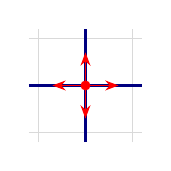
\begin{tikzpicture}[scale=0.6]
                    % Grid
                    \draw[step=1cm,gray!30,very thin] (-1.2,-1.2) grid (1.2,1.2);
                    % Cross strings
                    \draw[thick, NavyBlue] (-1.2,0) -- (1.2,0);
                    \draw[thick, NavyBlue] (0,-1.2) -- (0,1.2);
                    % Center
                    \fill[Red] (0,0) circle (3pt);
                    % Arrows
                    \draw[-{Stealth}, Red] (0,0) -- (-0.7,0);
                    \draw[-{Stealth}, Red] (0,0) -- (0.7,0);
                    \draw[-{Stealth}, Red] (0,0) -- (0,-0.7);
                    \draw[-{Stealth}, Red] (0,0) -- (0,0.7);
                \end{tikzpicture}
            \end{columns}
            This is called a \textit{\alert{partial differential equation}} or simply \textit{\alert{PDE}}.
        \end{block}
    }

    % 5. STEP 4: LAPLACIAN (Replaces Step 3 visual slightly or sits below)
    % Using 'only' to swap the bottom equation for the final result
    \visible<5->{
        \vspace{-0.2cm}
        \begin{alertblock}{Poisson's Equation (Arbitrary Dimension)}
%            Summing partials over all dimensions $x_i$:
            \begin{equation*}
                \boxed{ -\Delta u = f } \quad \text{where}\quad \Delta u \defeq \sum_{i=1}^d \frac{\partial^2 u}{\partial x_i^2}
            \end{equation*}
        \end{alertblock}
    }

\end{frame}

\begin{frame}{What does it mean to \textit{\alert{solve}} a PDE?}
% 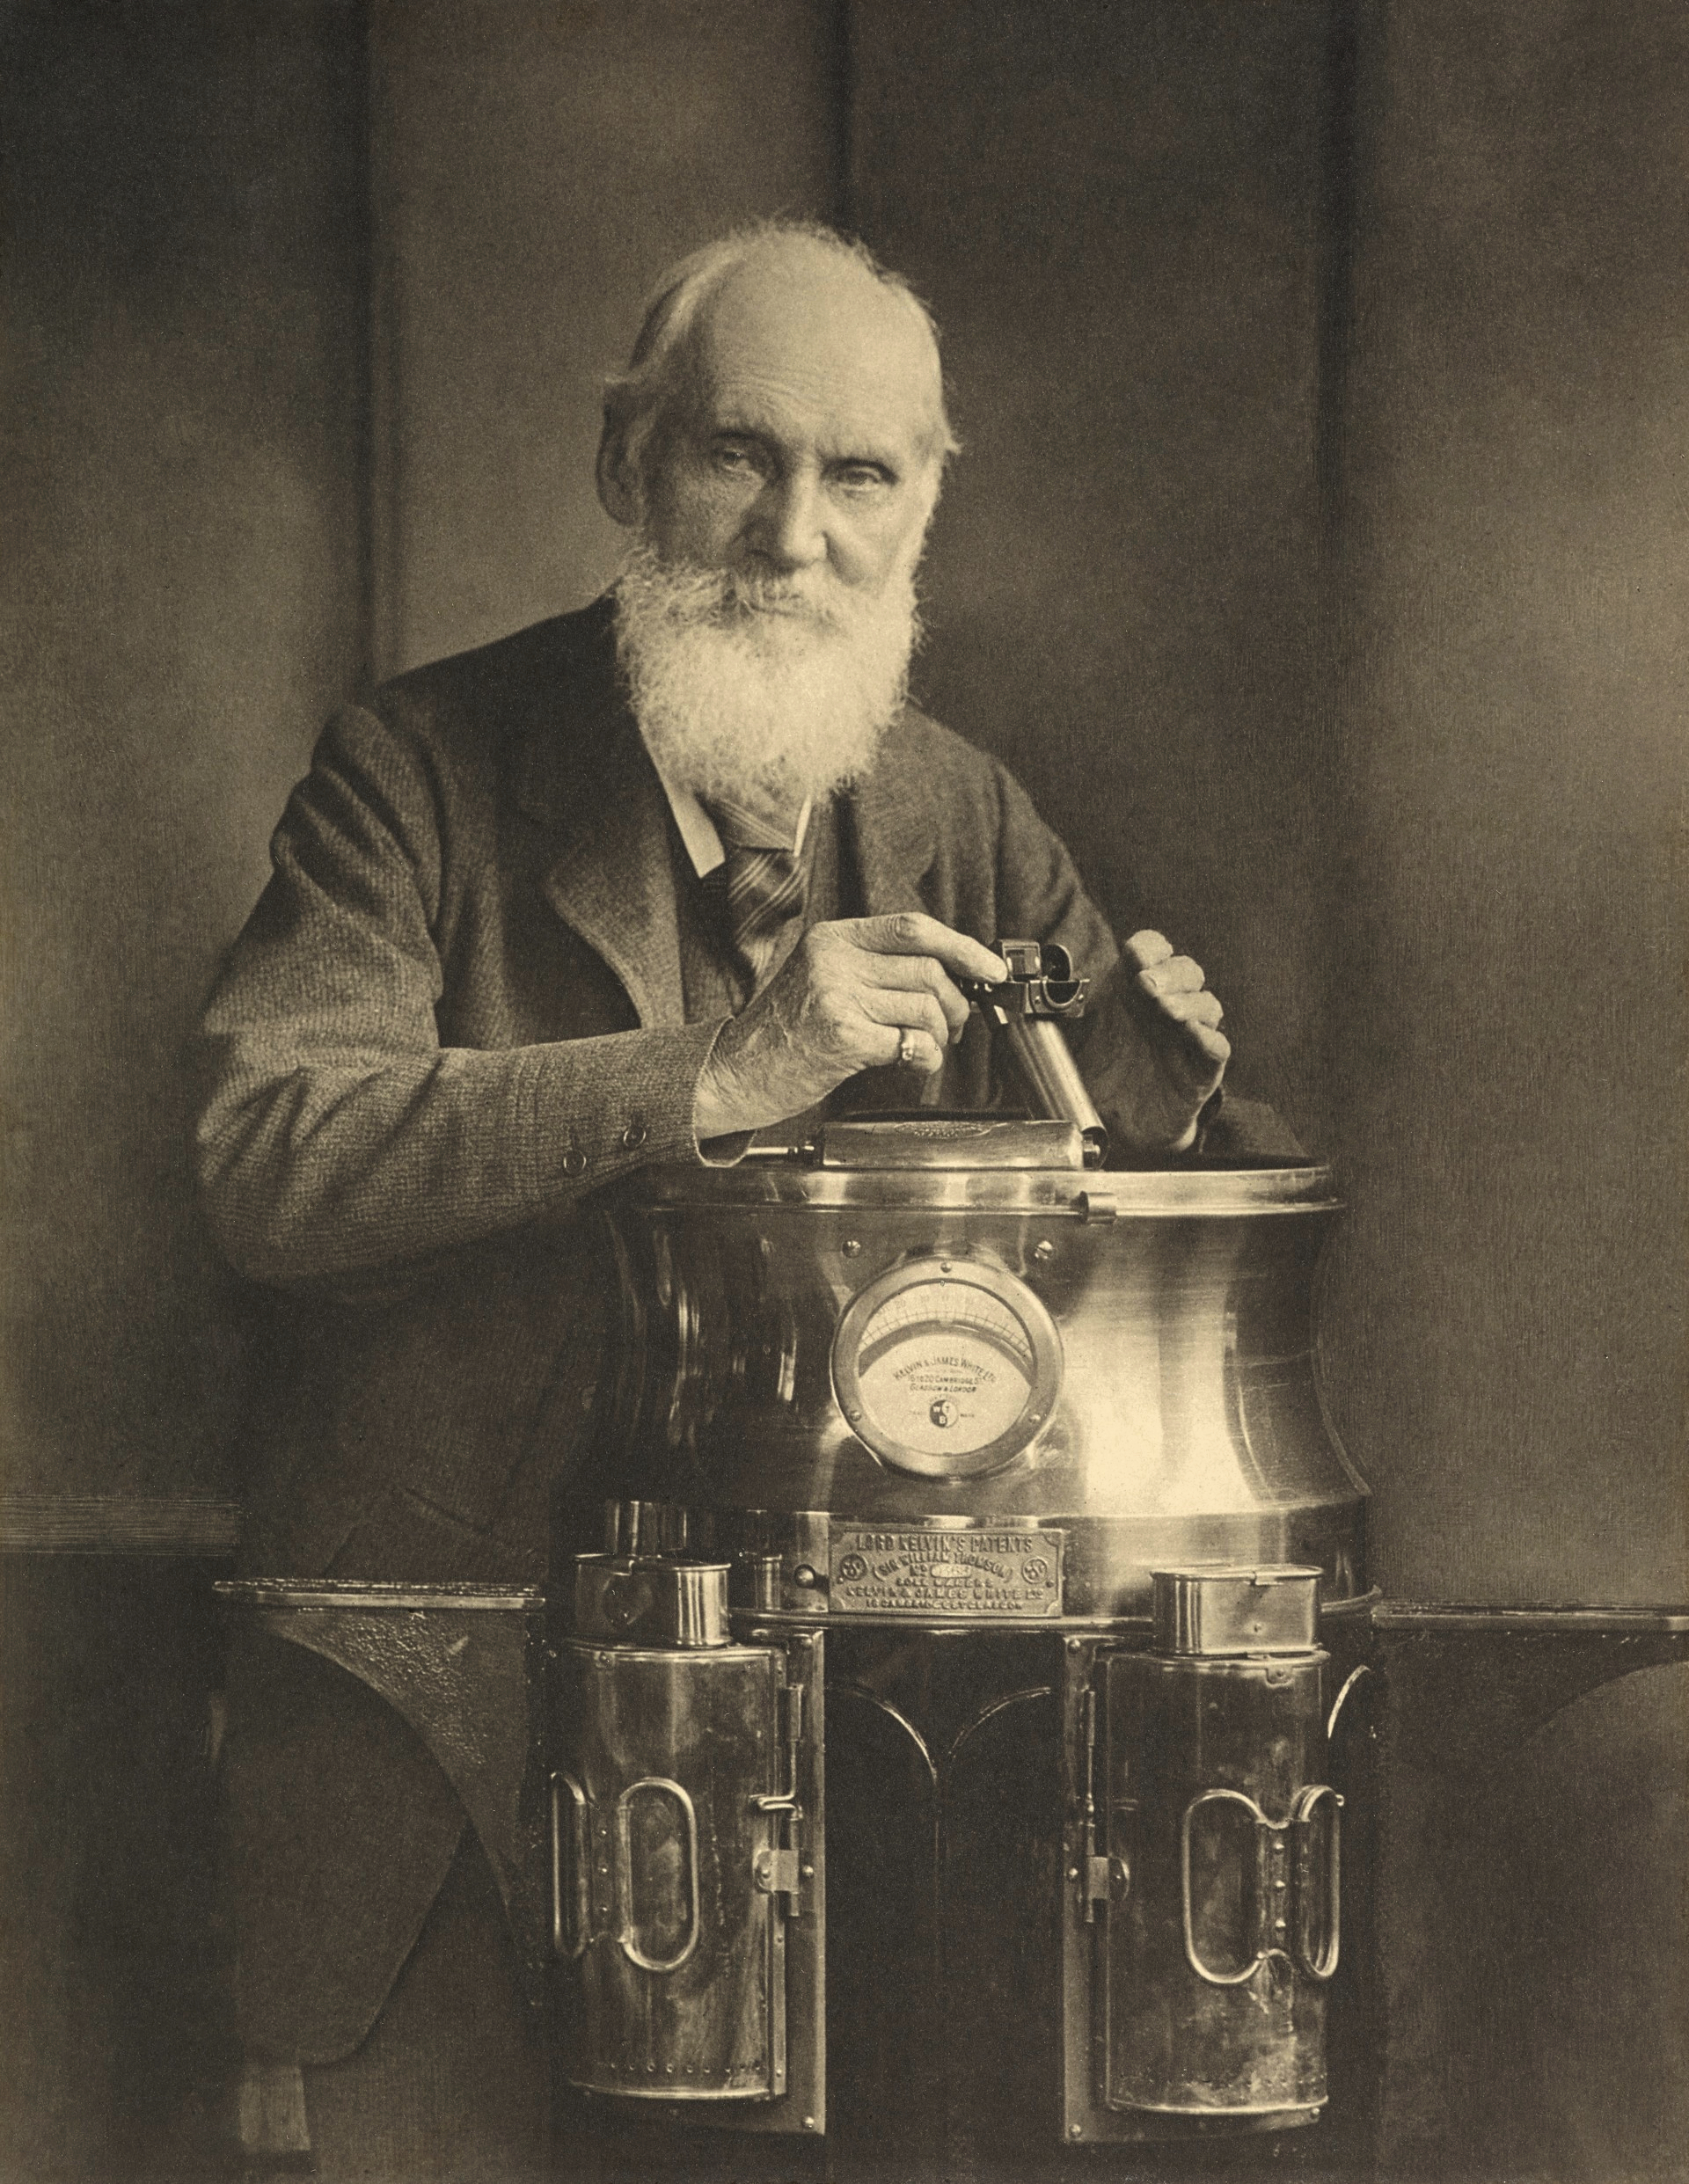
\includegraphics[width=\linewidth]{figures/kelvin.jpg}
%    \captionof*{figure}{\tiny W. Thomson}
%    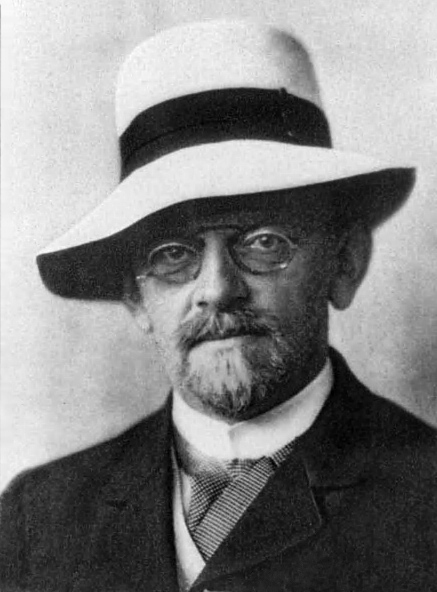
\includegraphics[width=\linewidth]{figures/Hilbert.jpg}
%    \captionof*{figure}{\tiny \alert{D. Hilbert}}
%    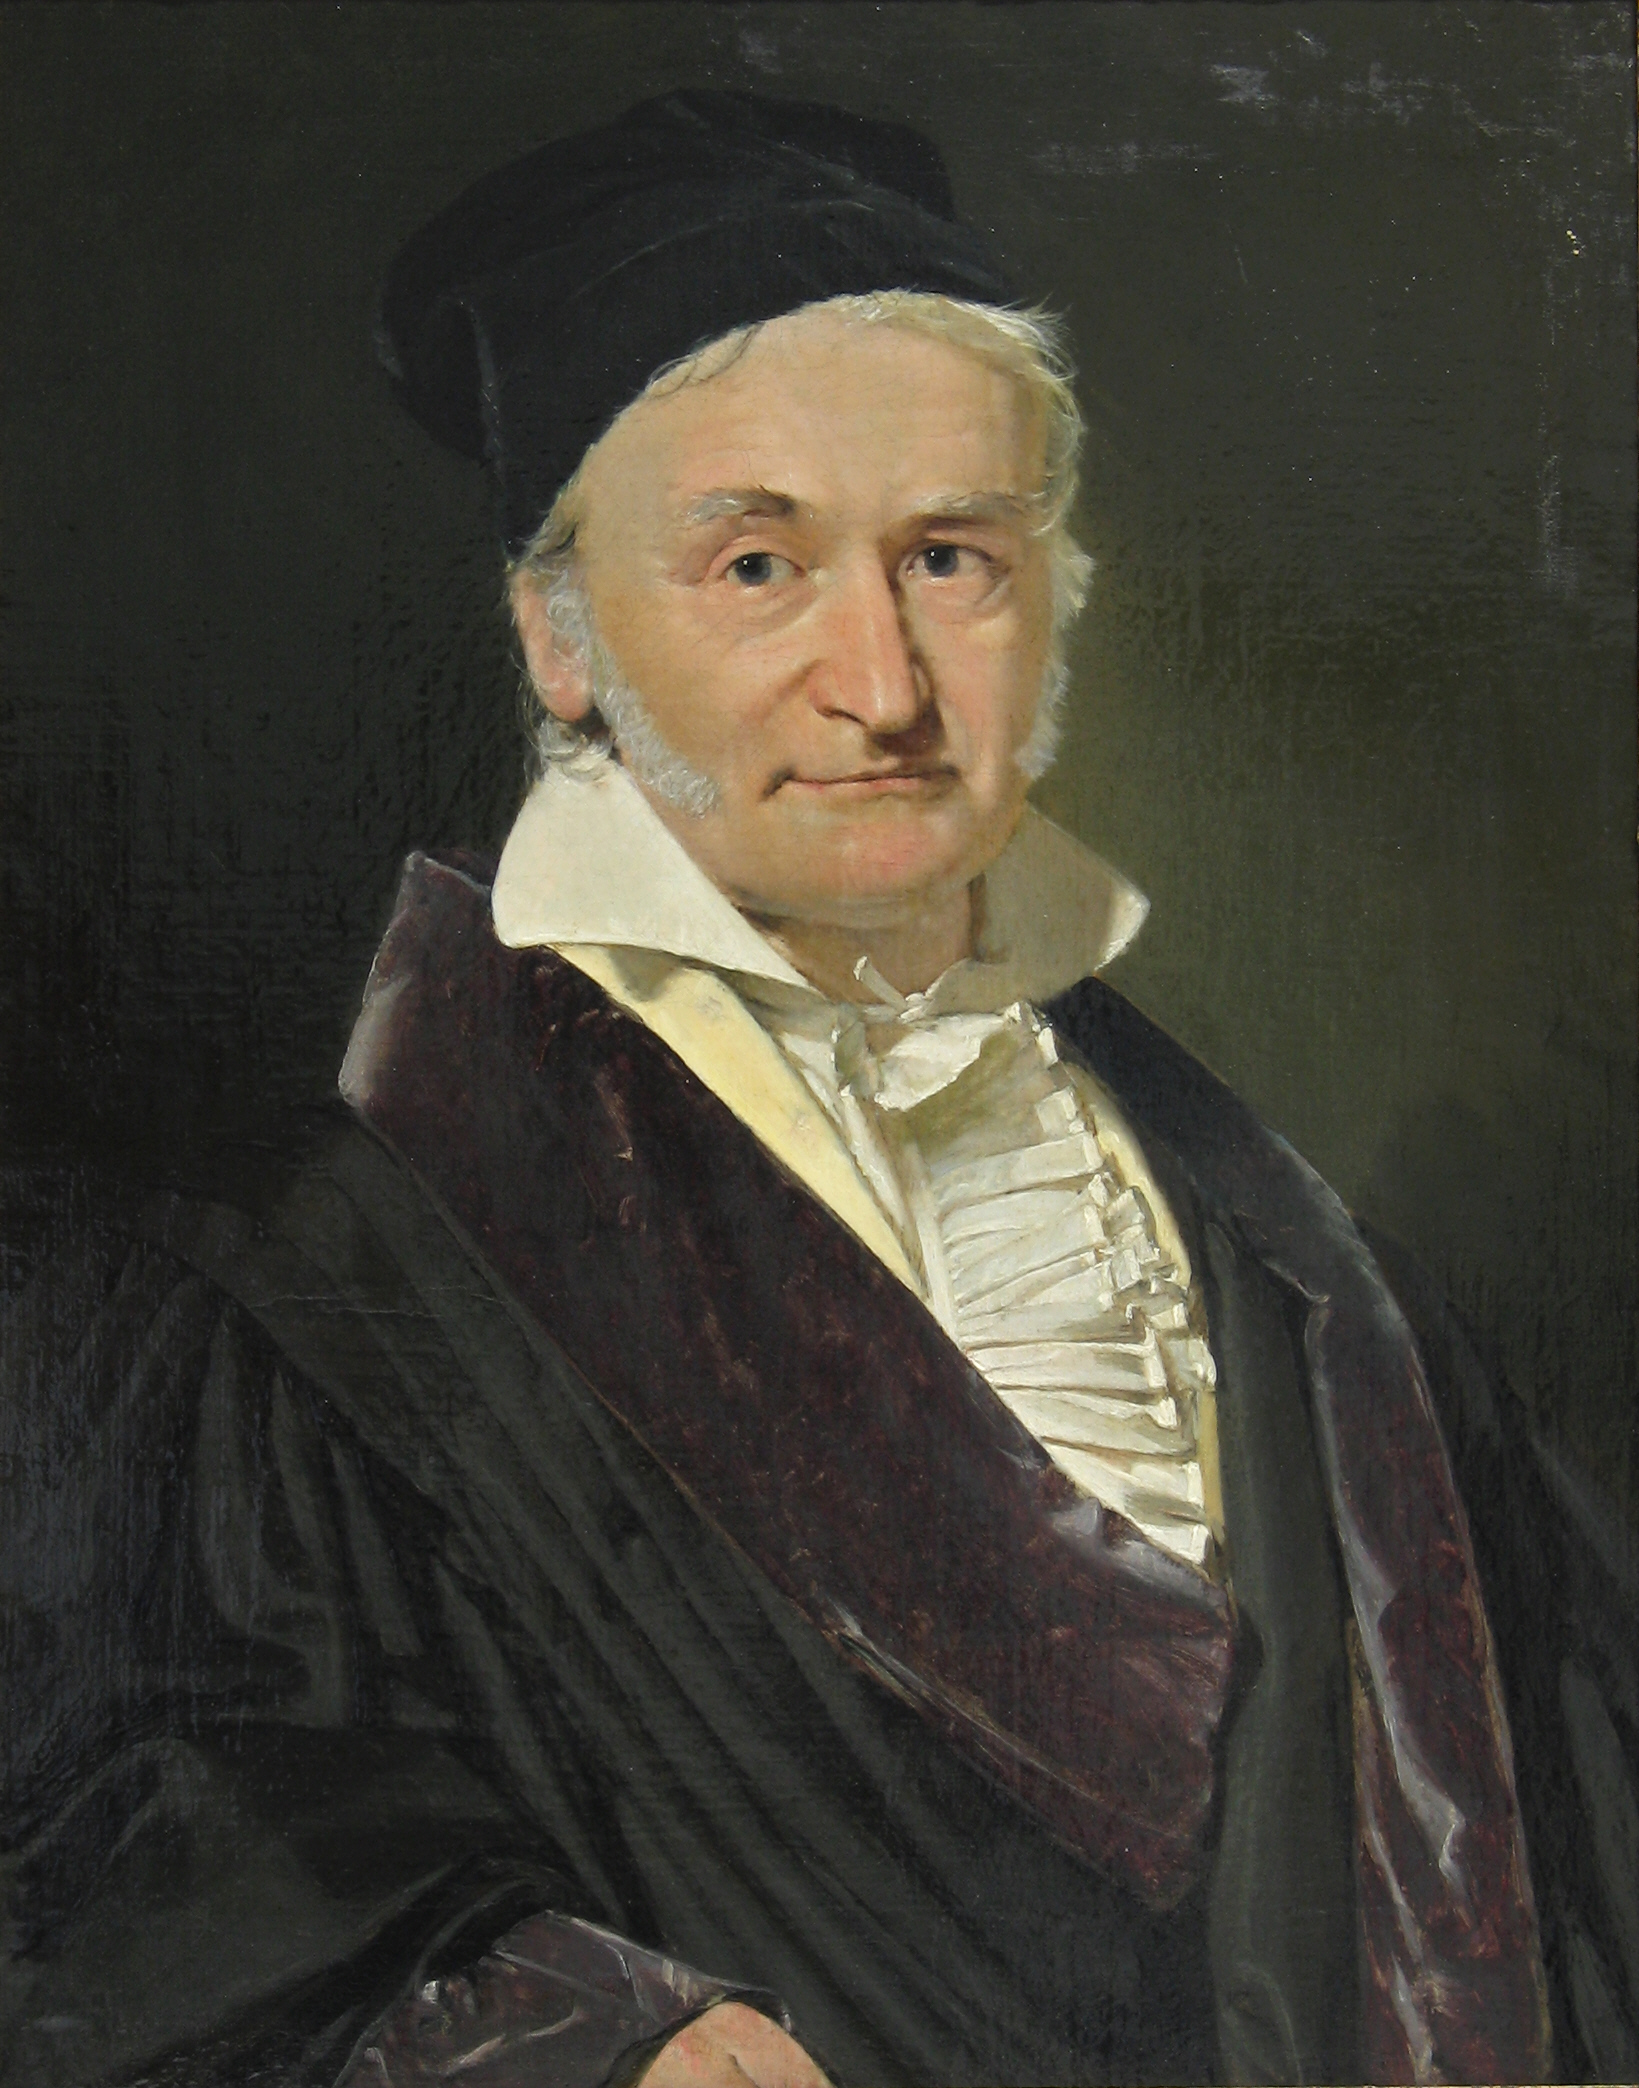
\includegraphics[width=\linewidth]{figures/gauss.jpg}
%    \captionof*{figure}{\tiny C.F. Gau\ss }
%    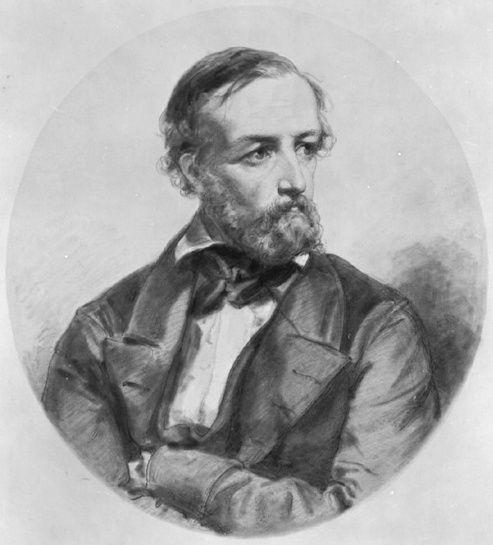
\includegraphics[width=\linewidth]{figures/dirichlet.jpg}
%    \captionof*{figure}{\tiny P.G.L. Dirichlet}
%    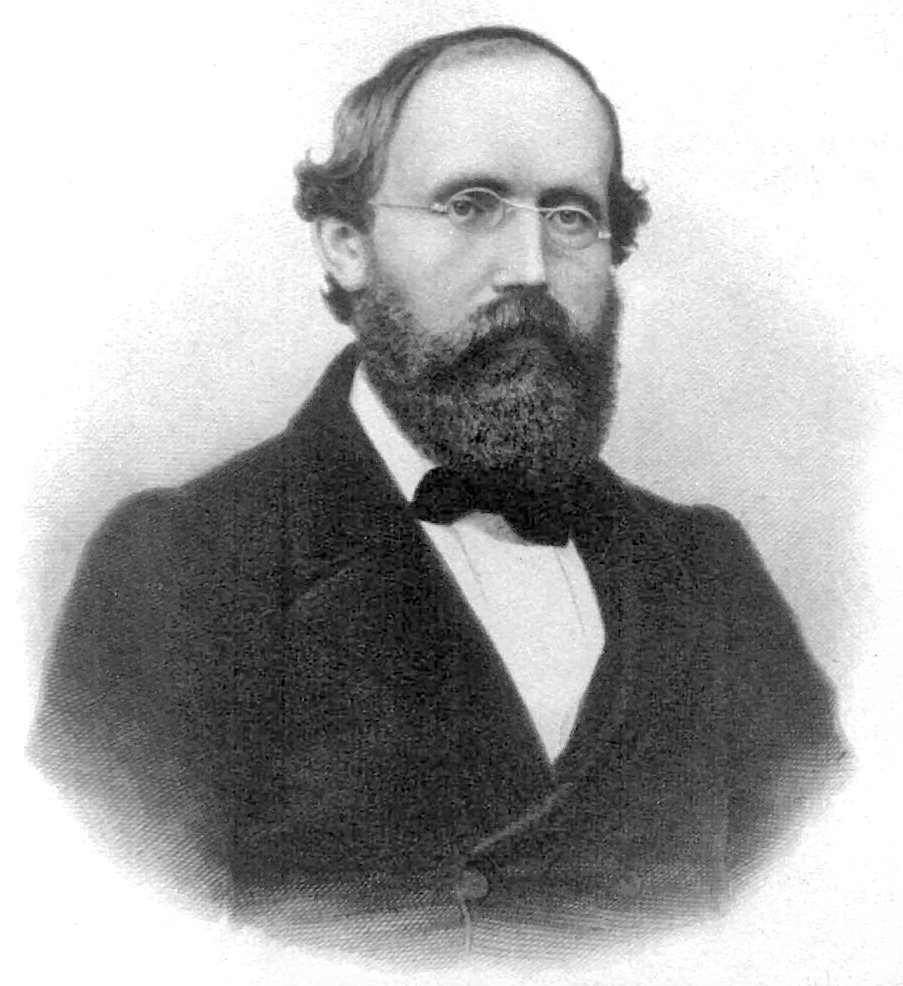
\includegraphics[width=\linewidth]{figures/riemann.jpg}
%    \captionof*{figure}{\tiny B. Riemann}
\visible<1->{
\centering When we solve Poisson's equation, we are looking for a \textit{\alert{function}} $u$.
}

 \only<2>{
\centering This (usually) cannot be done by pen and paper...
 }
\only<2>{\begin{figure}
    \centering
    % 1. KELVIN (W. Thomson)
    \begin{subfigure}[b]{0.18\textwidth}
        \centering
        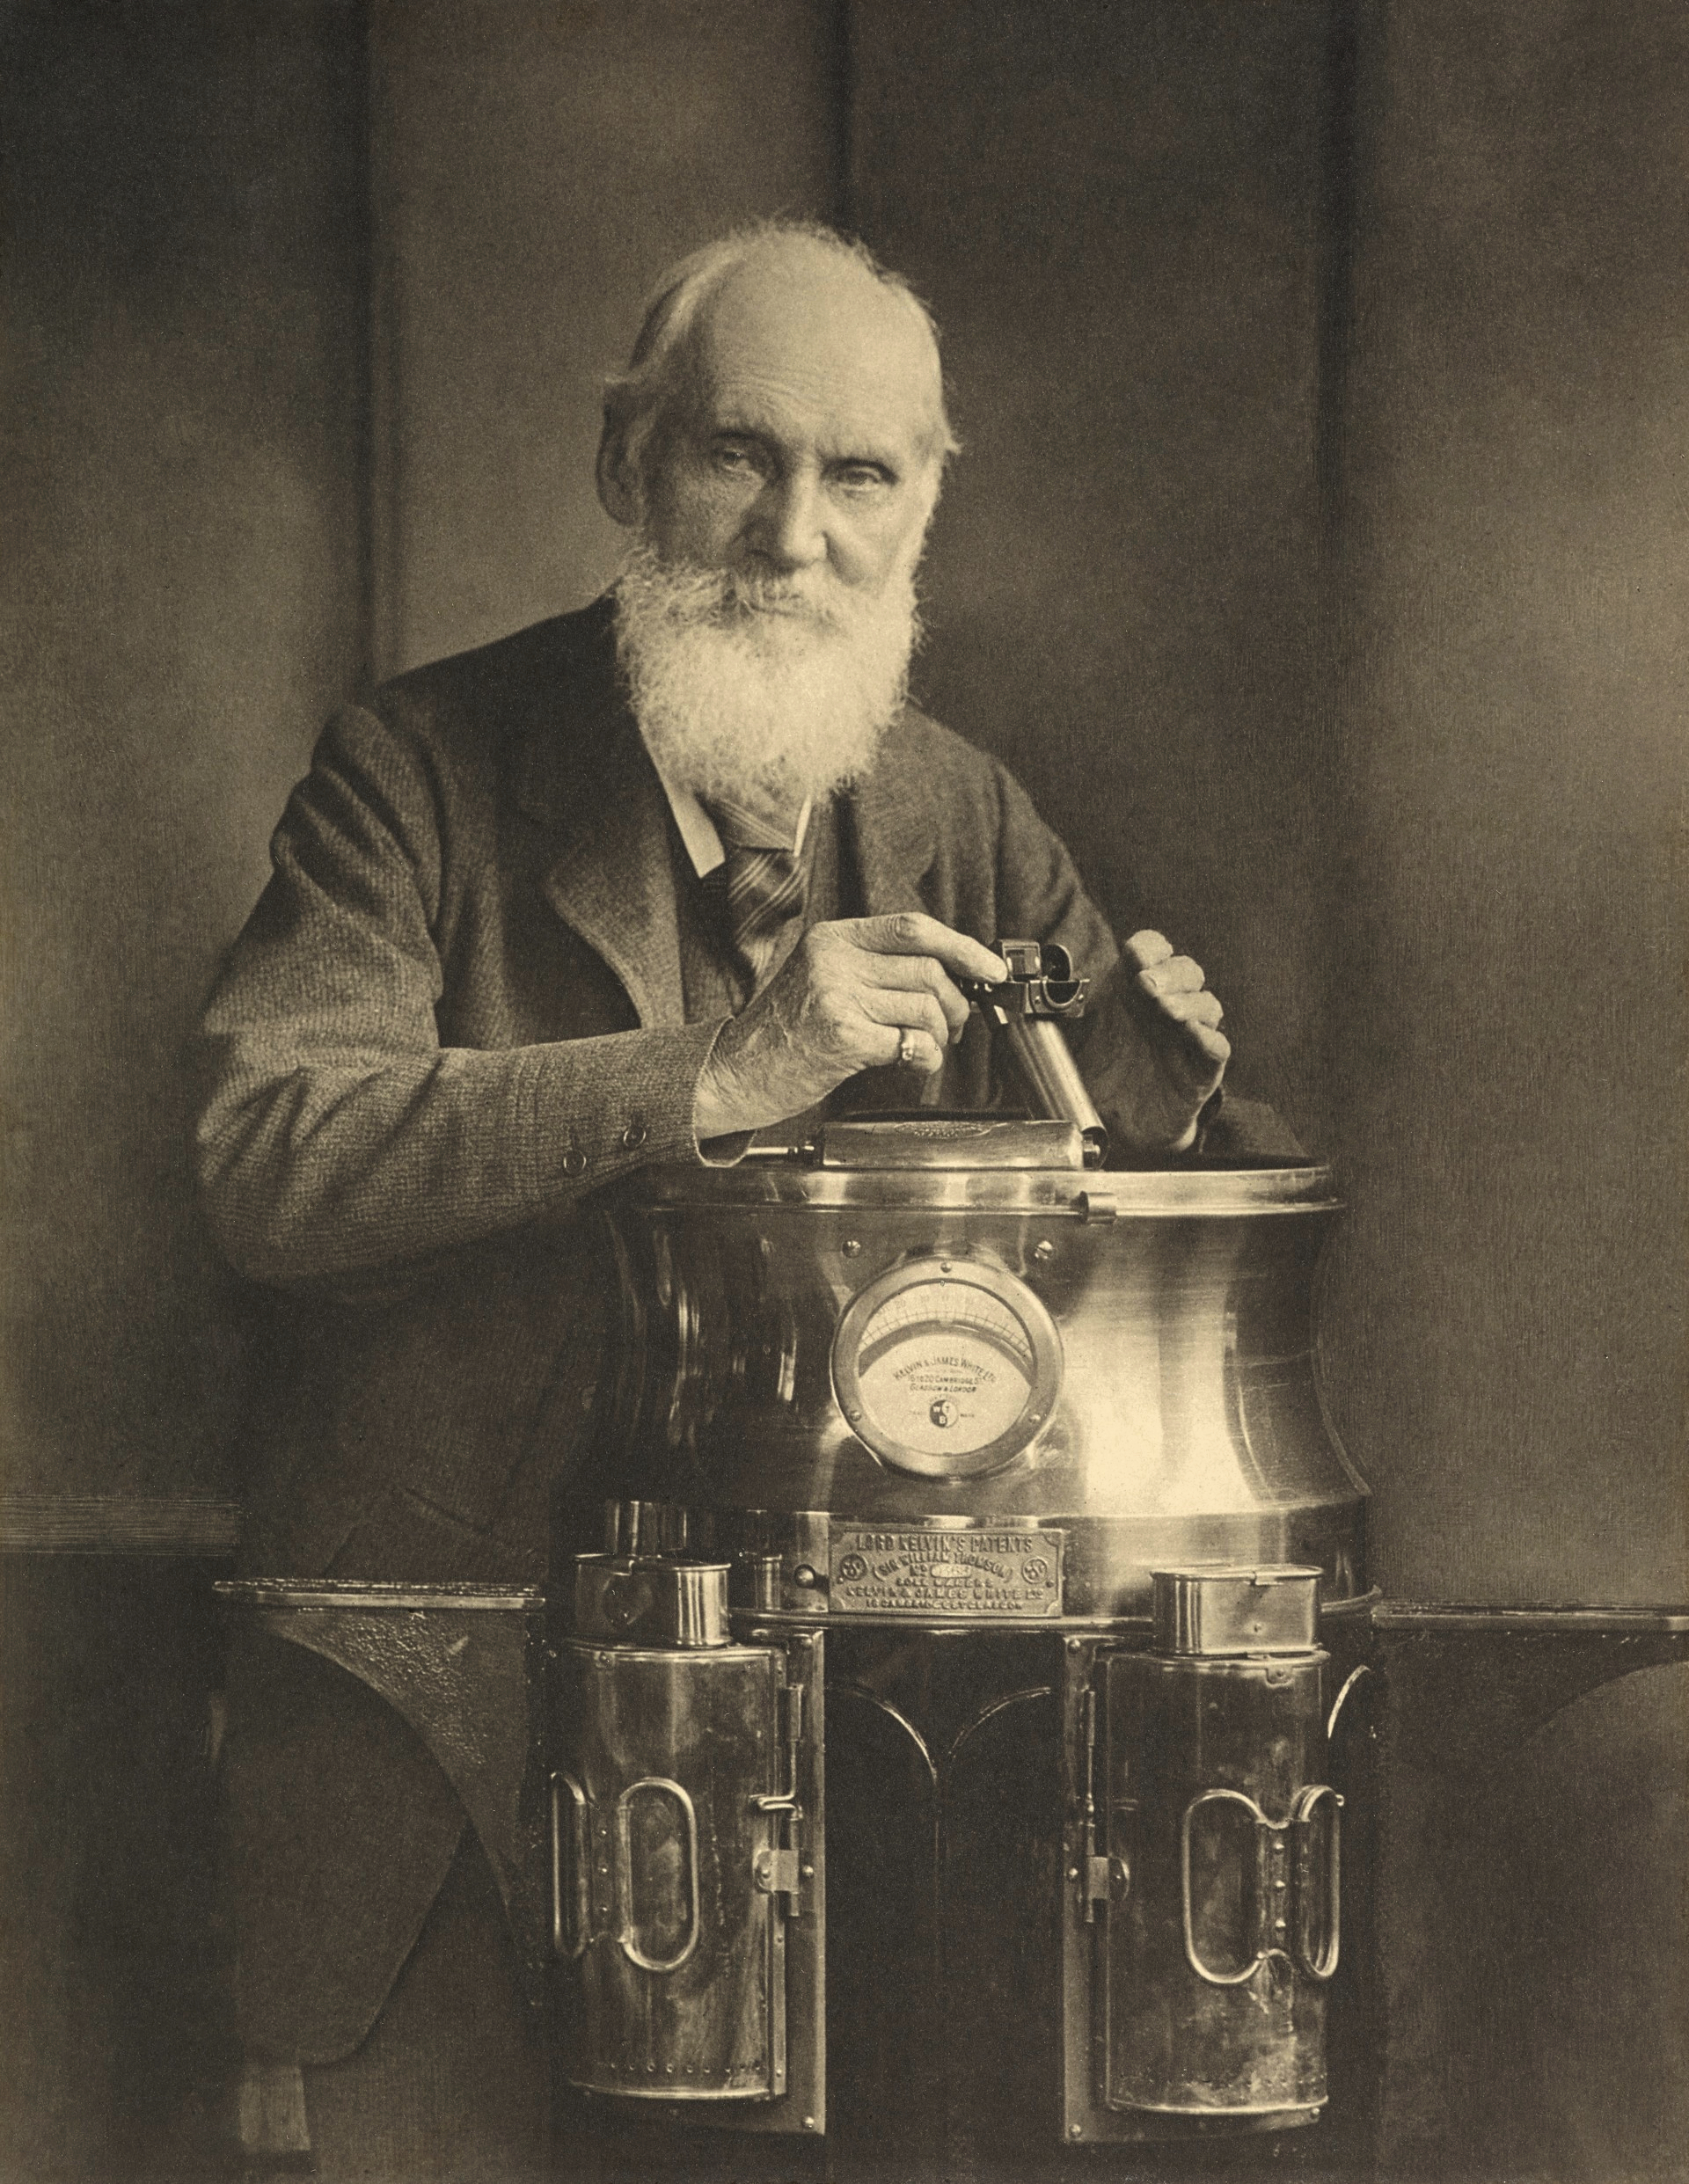
\includegraphics[width=\linewidth, height=0.20\textheight, keepaspectratio]{figures/kelvin.jpg}
        \caption*{\tiny W. Thomson}
    \end{subfigure}
    \hfill
    % 2. GAUSS
    \begin{subfigure}[b]{0.18\textwidth}
        \centering
        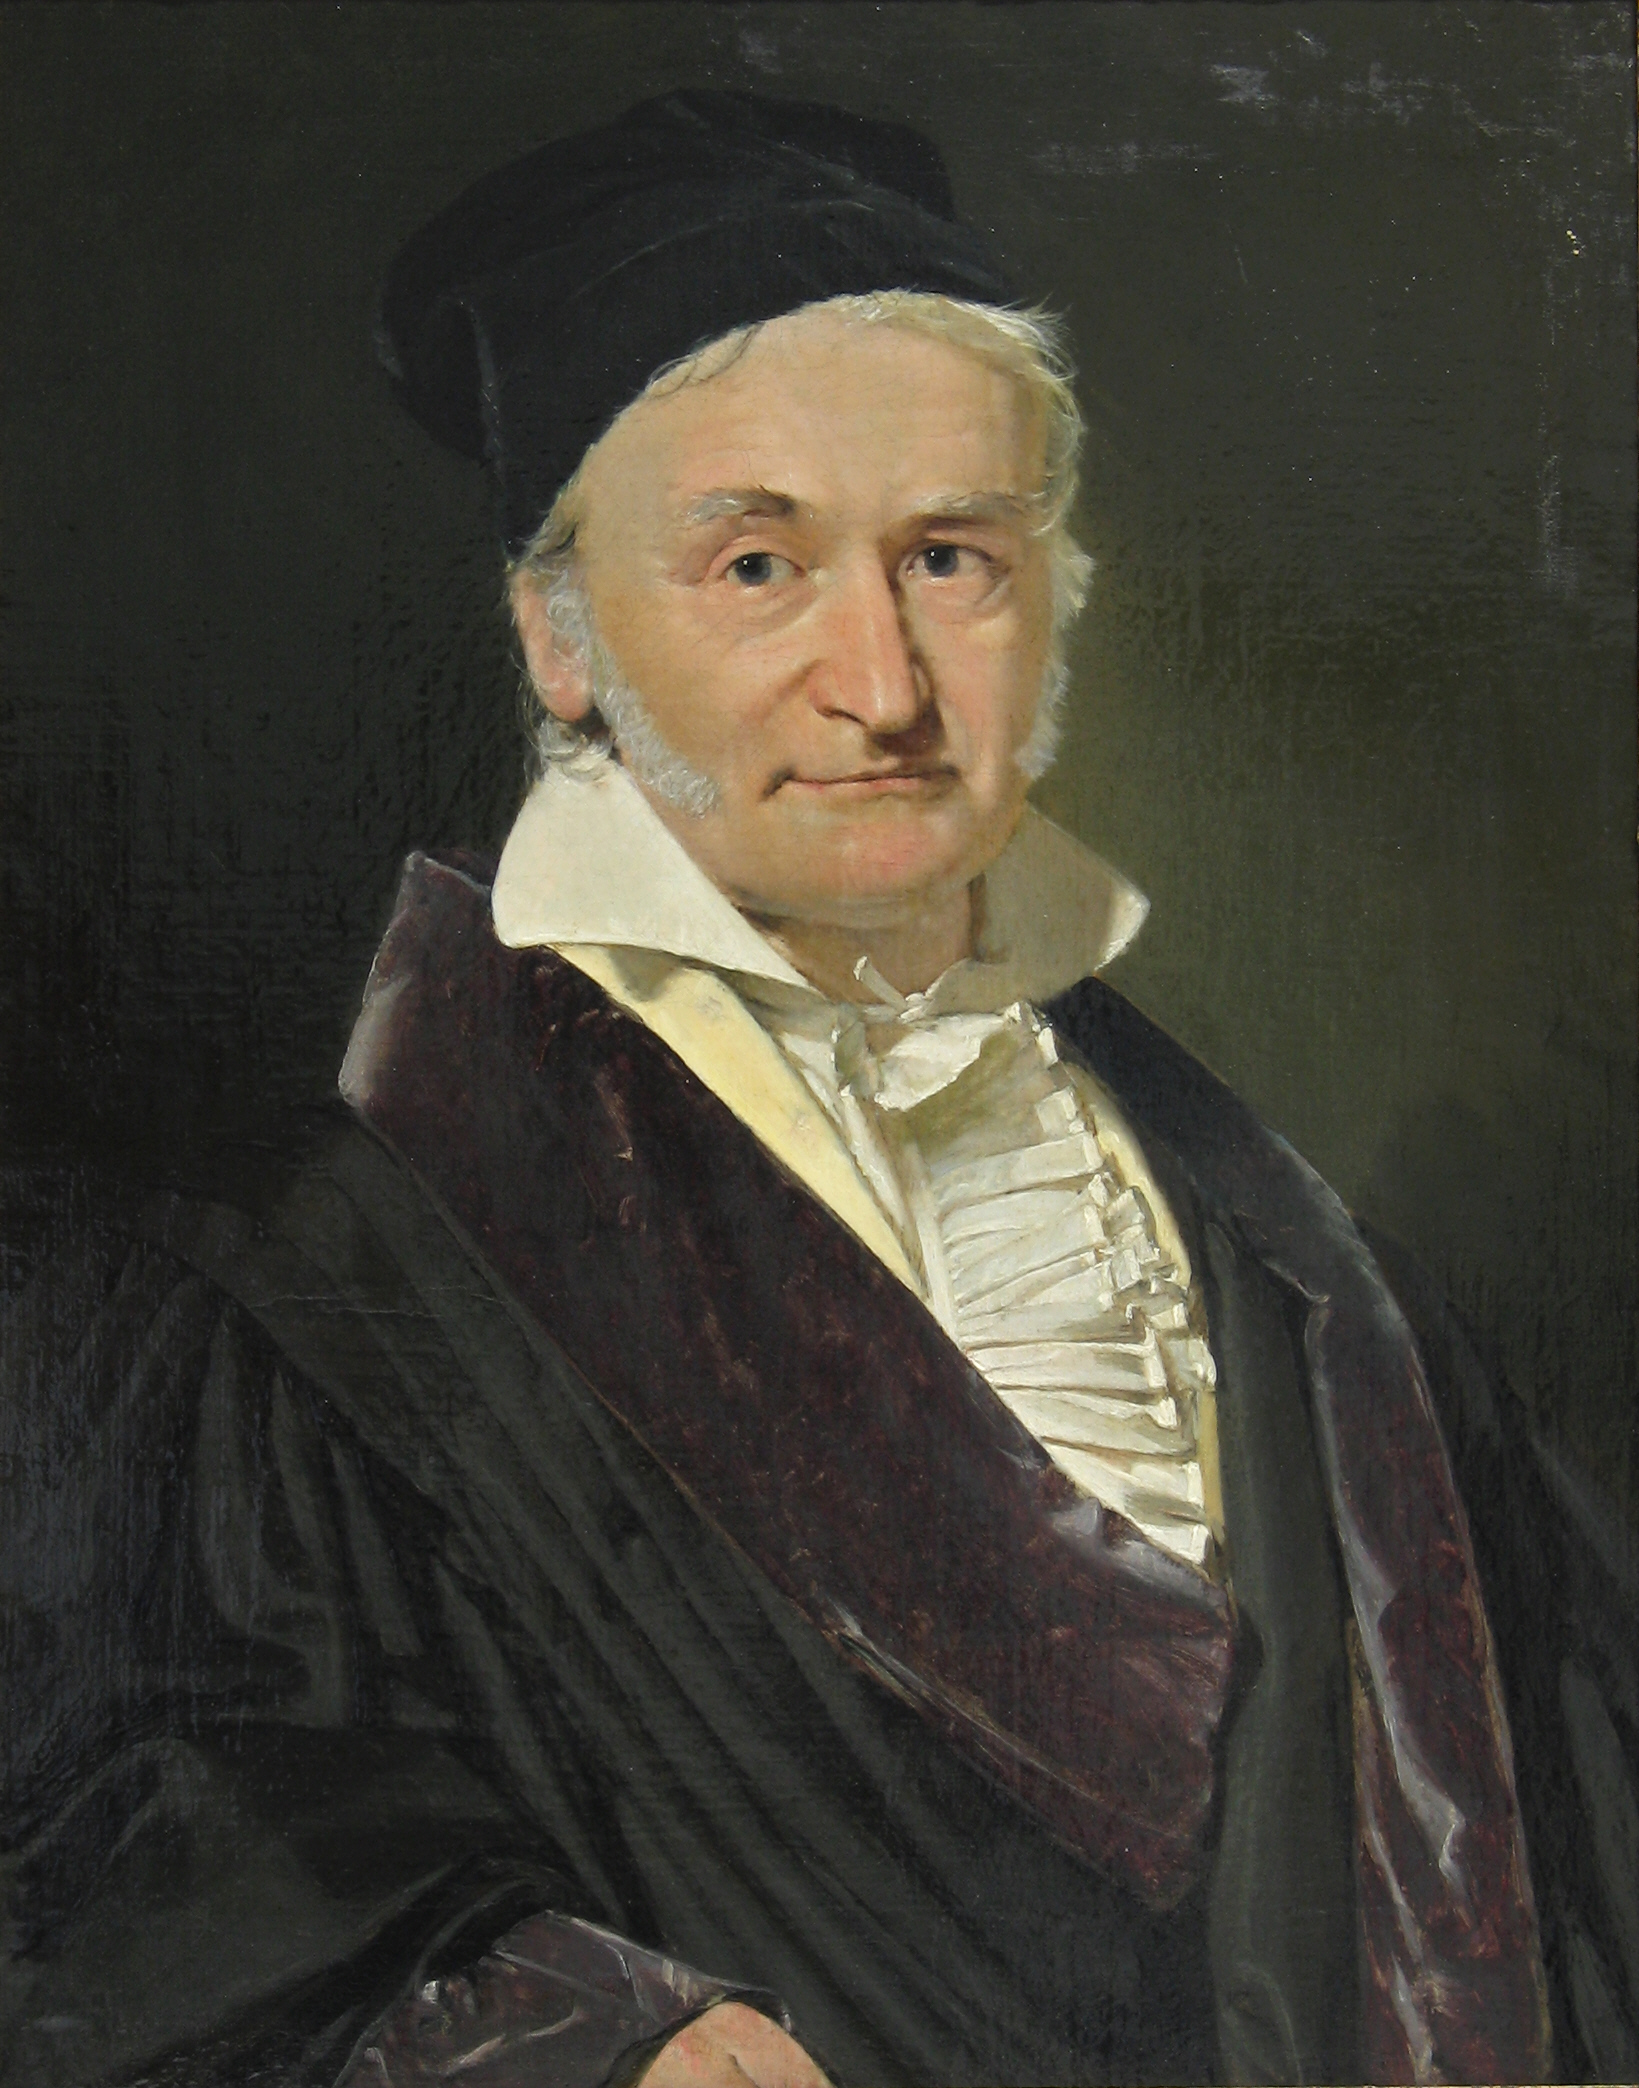
\includegraphics[width=\linewidth, height=0.20\textheight, keepaspectratio]{figures/gauss.jpg}
        \caption*{\tiny C.F. Gau\ss}
    \end{subfigure}
    \hfill
    % 3. DIRICHLET
    \begin{subfigure}[b]{0.18\textwidth}
        \centering
        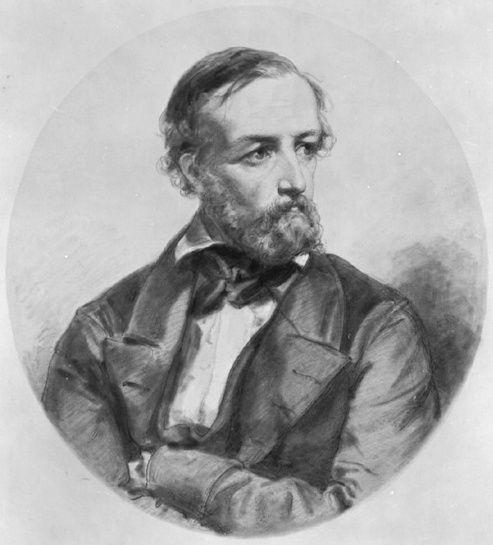
\includegraphics[width=\linewidth, height=0.20\textheight, keepaspectratio]{figures/dirichlet.jpg}
        \caption*{\tiny P.G.L. Dirichlet}
    \end{subfigure}
    \hfill
    % 4. RIEMANN
    \begin{subfigure}[b]{0.18\textwidth}
        \centering
        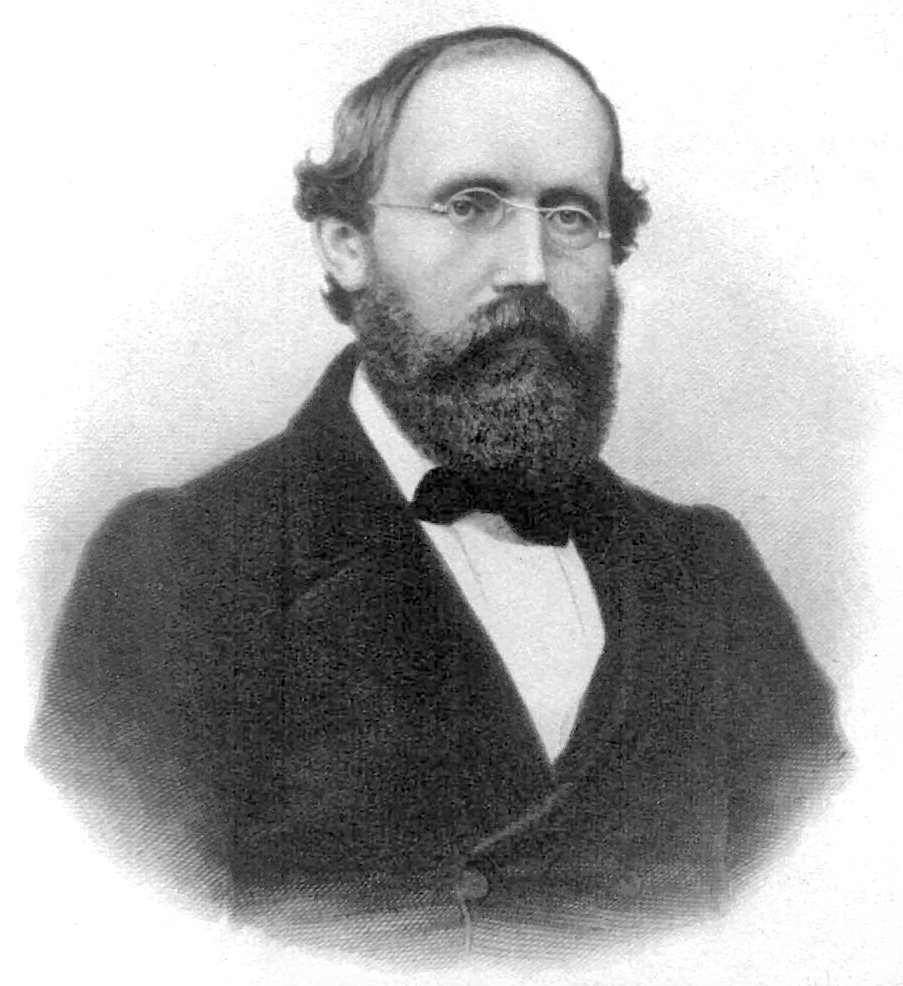
\includegraphics[width=\linewidth, height=0.20\textheight, keepaspectratio]{figures/riemann.jpg}
        \caption*{\tiny B. Riemann}
    \end{subfigure}
    \hfill
    % 5. HILBERT
    \begin{subfigure}[b]{0.18\textwidth}
        \centering
        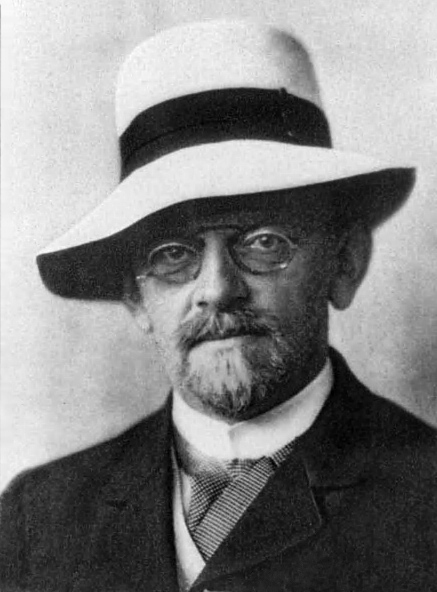
\includegraphics[width=\linewidth, height=0.20\textheight, keepaspectratio]{figures/Hilbert.jpg}
        \caption*{\tiny D. Hilbert}
    \end{subfigure}
\end{figure}}
 \only<3>{
\centering ...but it can be done with a computer\footnote{Using FEniCS for example}! Thanks, Jørgen!
 }
\only<3->{\begin{figure}
    \centering
    % 1. KELVIN (W. Thomson)
    \begin{subfigure}[b]{0.35\textwidth}
        \centering
        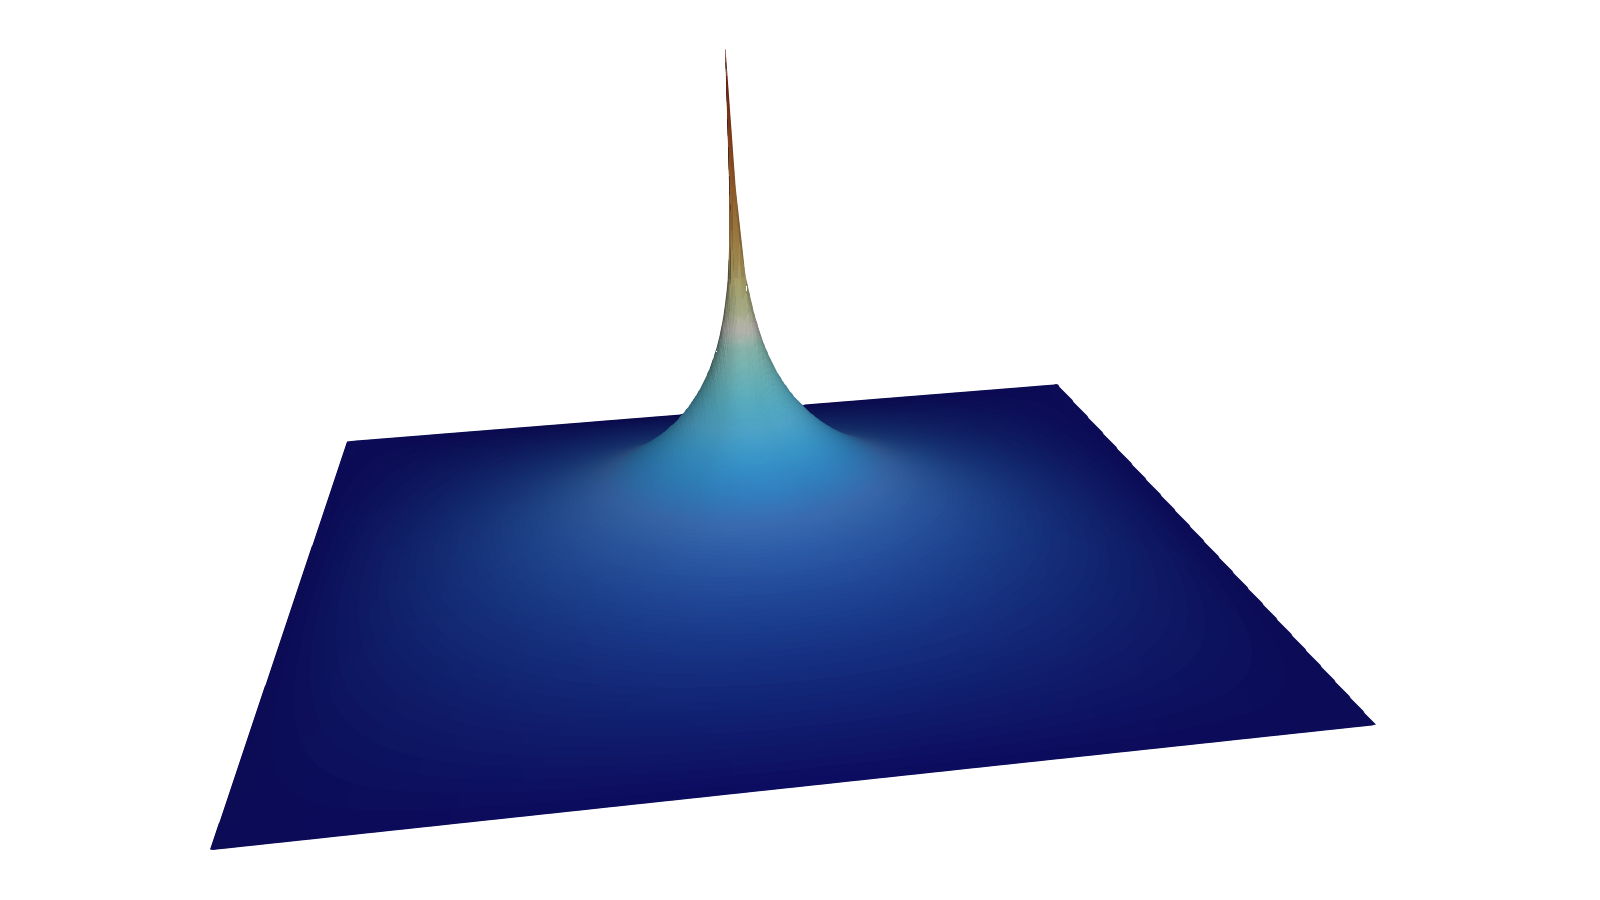
\includegraphics[width=\linewidth, height=\textheight, keepaspectratio]{figures/uh_point_source.png}
        \caption*{\tiny }
    \end{subfigure}
    \hfill
    % 2. GAUSS
    \begin{subfigure}[b]{0.18\textwidth}
        \centering
        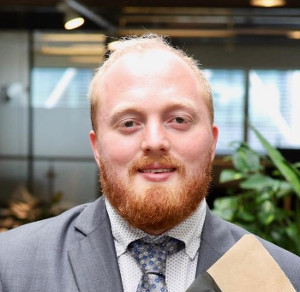
\includegraphics[width=\linewidth, height=\textheight, keepaspectratio]{figures/IMG_7528.png}
        \caption*{\tiny J.S. Dokken}
    \end{subfigure}
    \hfill
    % 3. DIRICHLET
    \begin{subfigure}[b]{0.35\textwidth}
        \centering
        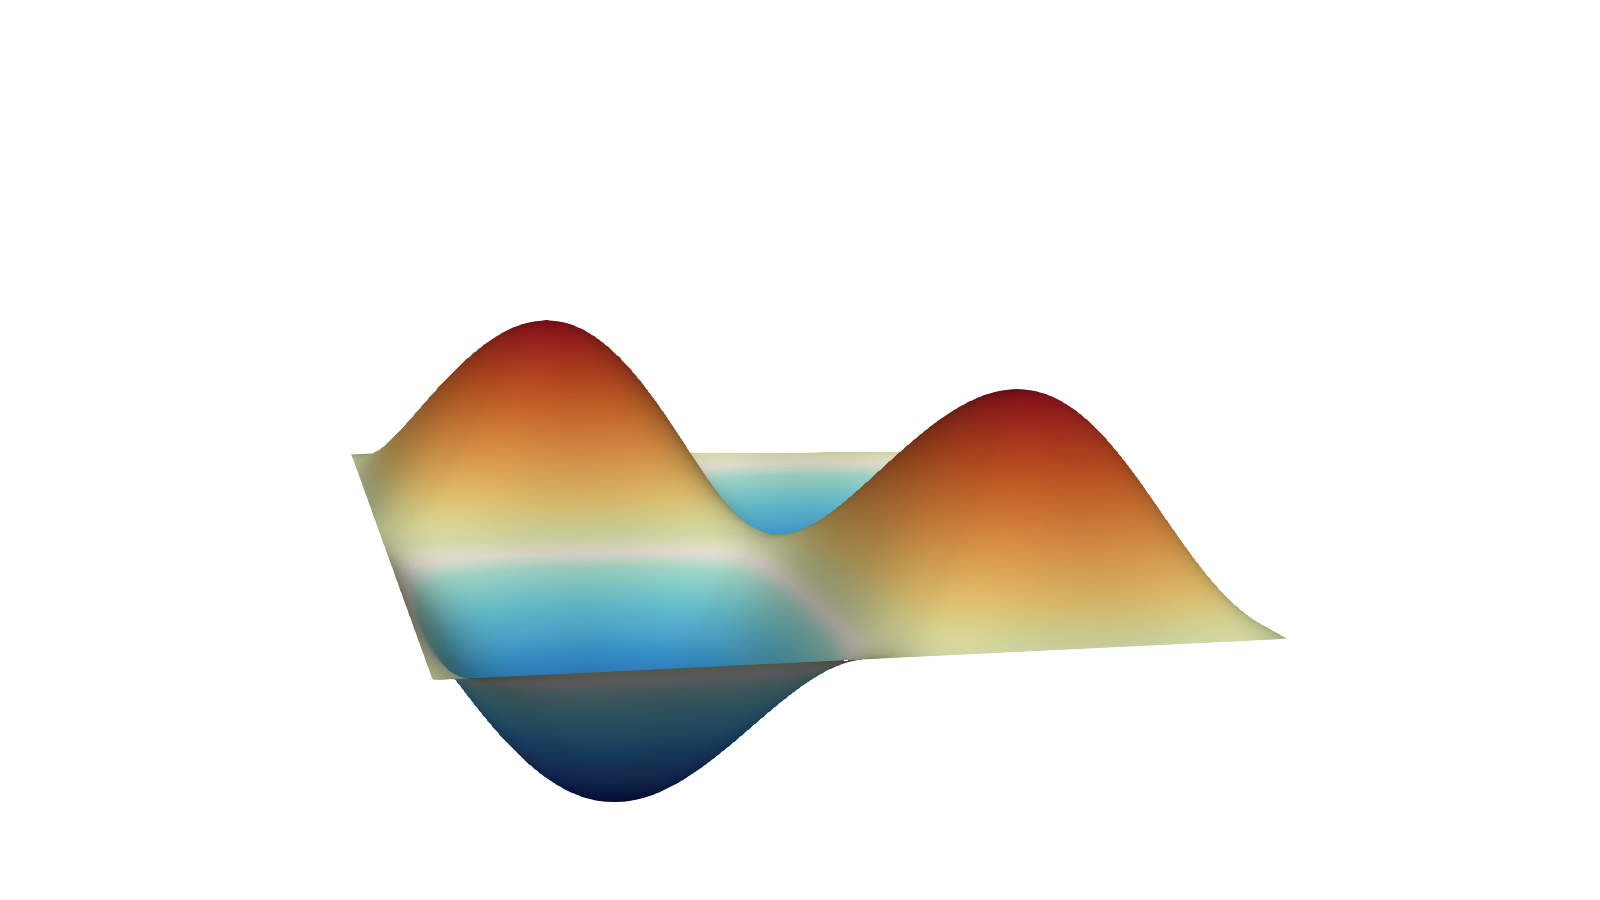
\includegraphics[width=\linewidth, height=\textheight, keepaspectratio]{figures/uh_poisson.png}
        \caption*{\tiny }
    \end{subfigure}
\end{figure}}
\end{frame}

\begin{frame}[plain,c]
%\frametitle{A first slide}
\hfill
\begin{center}
\Large So where do \alert{inequality constraints} come from?
\end{center}
\hfill
\end{frame}

\begin{frame}{So where do \alert{inequality constraints} come from?}

    \transfade[duration=0.5]<2->

% --- PERMANENT NAVIGATION HEADER ---
    \centering
    \footnotesize
    % Step 1: Highlighted on Slide 1, Gray otherwise
    \alt<1>{\textbf{\textcolor{NavyBlue}{1. Constraint}}}{\textcolor{gray!50}{1. Constraint}}
    \hspace{1em} $\to$ \hspace{1em}
    % Step 2: Highlighted on Slide 2
    \alt<2>{\textbf{\textcolor{NavyBlue}{2. Reaction}}}{\textcolor{gray!50}{2. Reaction}}
    \hspace{1em} $\to$ \hspace{1em}
    % Step 3: Highlighted on Slide 3
    \alt<3>{\textbf{\textcolor{NavyBlue}{3. Complementarity}}}{\textcolor{gray!50}{3. Complementarity}}
    \hspace{1em} $\to$ \hspace{1em}
    % Step 4: Highlighted on Slide 4
    \alt<4>{\textbf{\textcolor{NavyBlue}{4. Variational Inequality}}}{\textcolor{gray!50}{4. Variational Inequality}}
    
    \vspace{0.3cm}
    % -----------------------------------

    % 1. THE OBSTACLE (Physical Setup)
    \only<1>{
        \begin{block}{Step 1: The Obstacle Problem}
            \begin{columns}
                \column{0.65\textwidth}
                \small
                Suppose the string cannot penetrate a rigid obstacle $\psi(x)$.
                \begin{itemize}
                    \item We require \textbf{admissibility}: $u(x) \ge \psi(x)$.
                    \item Gravity $f$ pulls the string down onto the obstacle.
                \end{itemize}
                
                \column{0.3\textwidth}
                \centering
                % TikZ: String hitting an obstacle
                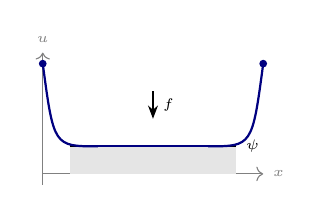
\begin{tikzpicture}[scale=0.7]
                    % Axis
                    \draw[->, gray] (-2, -1.2) -- (-2, 1.2) node[above] {\tiny $u$};
                    \draw[->, gray] (-2, -1) -- (2, -1) node[right] {\tiny $x$};
                    
                    % Obstacle (Table)
                    \fill[gray!20] (-1.5, -0.5) rectangle (1.5, -1);
                    \draw[thick, black] (-1.5, -0.5) -- (1.5, -0.5) node[right] {\tiny $\psi$};
                    
                    % String (Fixed ends, sagging, flat bottom)
                    \draw[thick, NavyBlue] (-2, 1) .. controls (-1.8, -0.5) .. (-1, -0.5); % Left drop
                    \draw[thick, NavyBlue] (-1, -0.5) -- (1, -0.5); % Contact patch
                    \draw[thick, NavyBlue] (1, -0.5) .. controls (1.8, -0.5) .. (2, 1); % Right rise
                    \fill[NavyBlue] (-2,1) circle (2pt);
                    \fill[NavyBlue] (2,1) circle (2pt);
                    
                    % Load
                    \draw[-{Stealth}, black] (0, 0.5) -- (0, 0) node[midway, right] {\tiny $f$};
                \end{tikzpicture}
            \end{columns}
        \end{block}
    }

    % 2. REACTION FORCES
    \only<2>{
        \begin{block}{Step 2: A Reaction Force}
            Where the string touches the obstacle ($u = \psi$), the obstacle pushes back with a \textbf{reaction force} $\lambda \ge 0$ to prevent penetration.
            \begin{equation*}
                -\frac{\partial^2 u}{\partial x_i^2}(x) = f(x) + \underbrace{\lambda(x)}_{\text{Reaction}}
            \end{equation*}
        \end{block}
    }

    % 3. COMPLEMENTARITY
    \only<3>{
        \begin{block}{Step 3: Complementarity}
            The physics implies a strict "either-or" condition:
            \begin{itemize}
                \item \textbf{Free Region} ($u > \psi$): No contact $\implies \lambda = 0$ 
                \alert{(No Reaction Force)} $\implies -\frac{\partial^2 u}{\partial x_i^2} = f$ \alert{(Back to Poisson)}.
                \item \textbf{Contact Region} ($u = \psi$): Contact $\implies \lambda \ge 0$ \alert{(Reaction Force)}$\implies -\frac{\partial^2 u}{\partial x_i^2} \ge f$ \alert{(???)}.
            \end{itemize}
%            \[
% \text{Ideally: } \quad ( -u'' - f ) \cdot (u - \psi) = 0 \quad \text{with } u \ge \psi, \ -u'' \ge f
%            \]
        \end{block}
    }

    % 4. VARIATIONAL INEQUALITY
    \only<4>{
        \begin{alertblock}{Step 4: The Variational Inequality}
            Multiplying by a test function $(v - u)$ where $v \ge \psi$ eliminates the unknown reaction force $\lambda$ (since $\lambda \cdot (v-u) \ge 0$):
            \begin{equation*}
                \boxed{ \langle -\Delta u,  v - u \rangle \ge \langle f, v - u\rangle \quad \forall v \in \mathcal{K} }
            \end{equation*}
            where $\mathcal{K} = \{ v : v \ge \psi \text{ a.e.} \}$.
        \end{alertblock}
    }

\end{frame}

\begin{frame}\frametitle{Pointwise bounds are ubiquitous\footnote{\tiny All examples from Dokken, Farrell, Keith, Papadopoulos, Surowiec (2025)}}
\captionsetup[subfigure]{labelformat=empty} % Disable subfigure labels

\begin{figure}
    \centering
    \begin{subcaptionbox}{$K = \{u \ge \phi\}$}[0.3\textwidth]
        {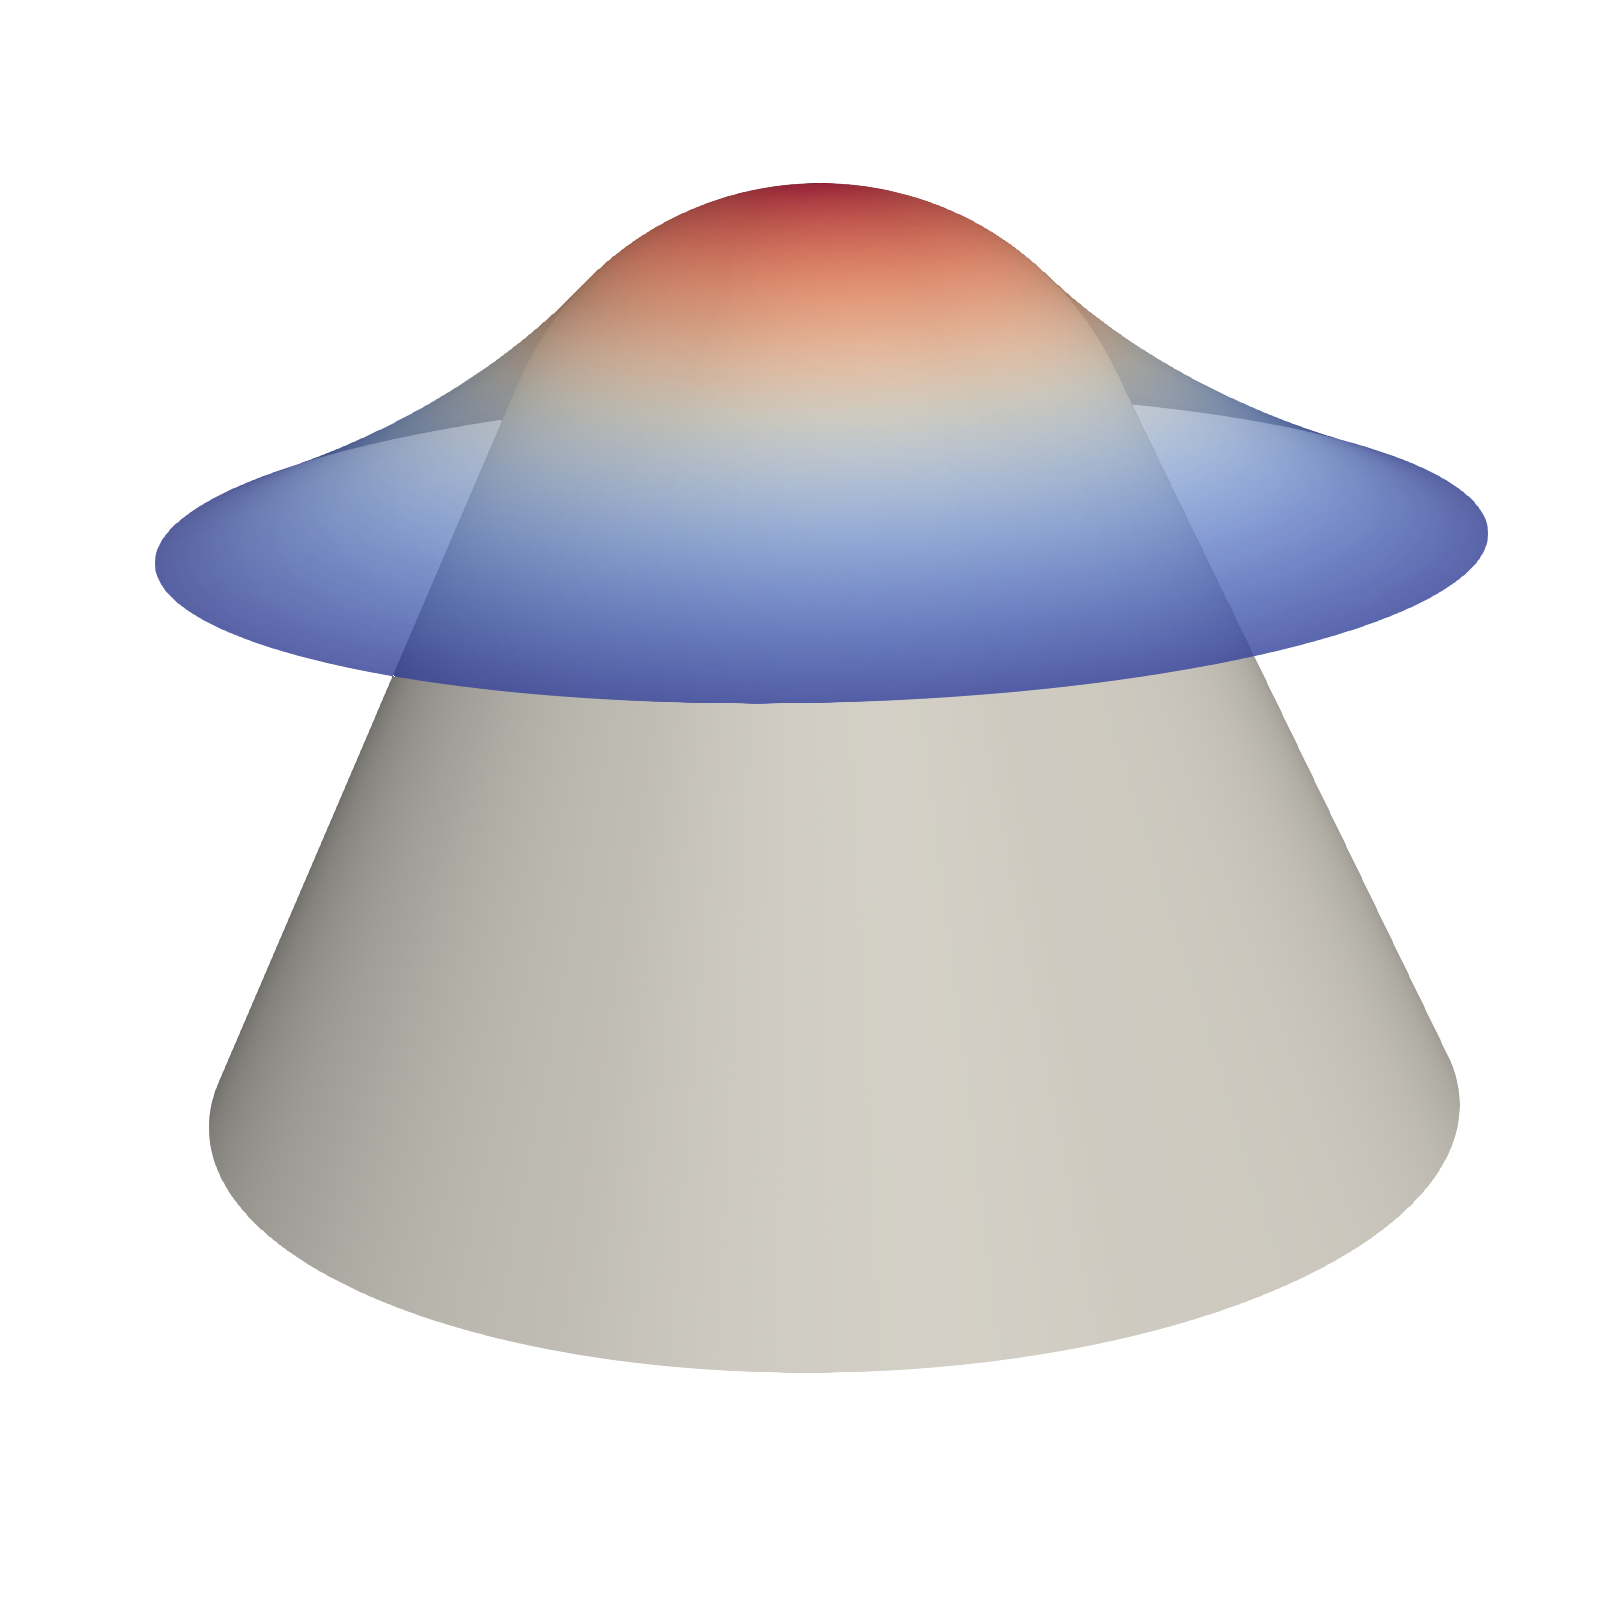
\includegraphics[width=0.5\linewidth]{figures/obstacle_new.png}}
    \end{subcaptionbox}
    \hfill
    \begin{subcaptionbox}{$K = \{\gamma(u) \cdot n \ge 0\}$}[0.3\textwidth]
        {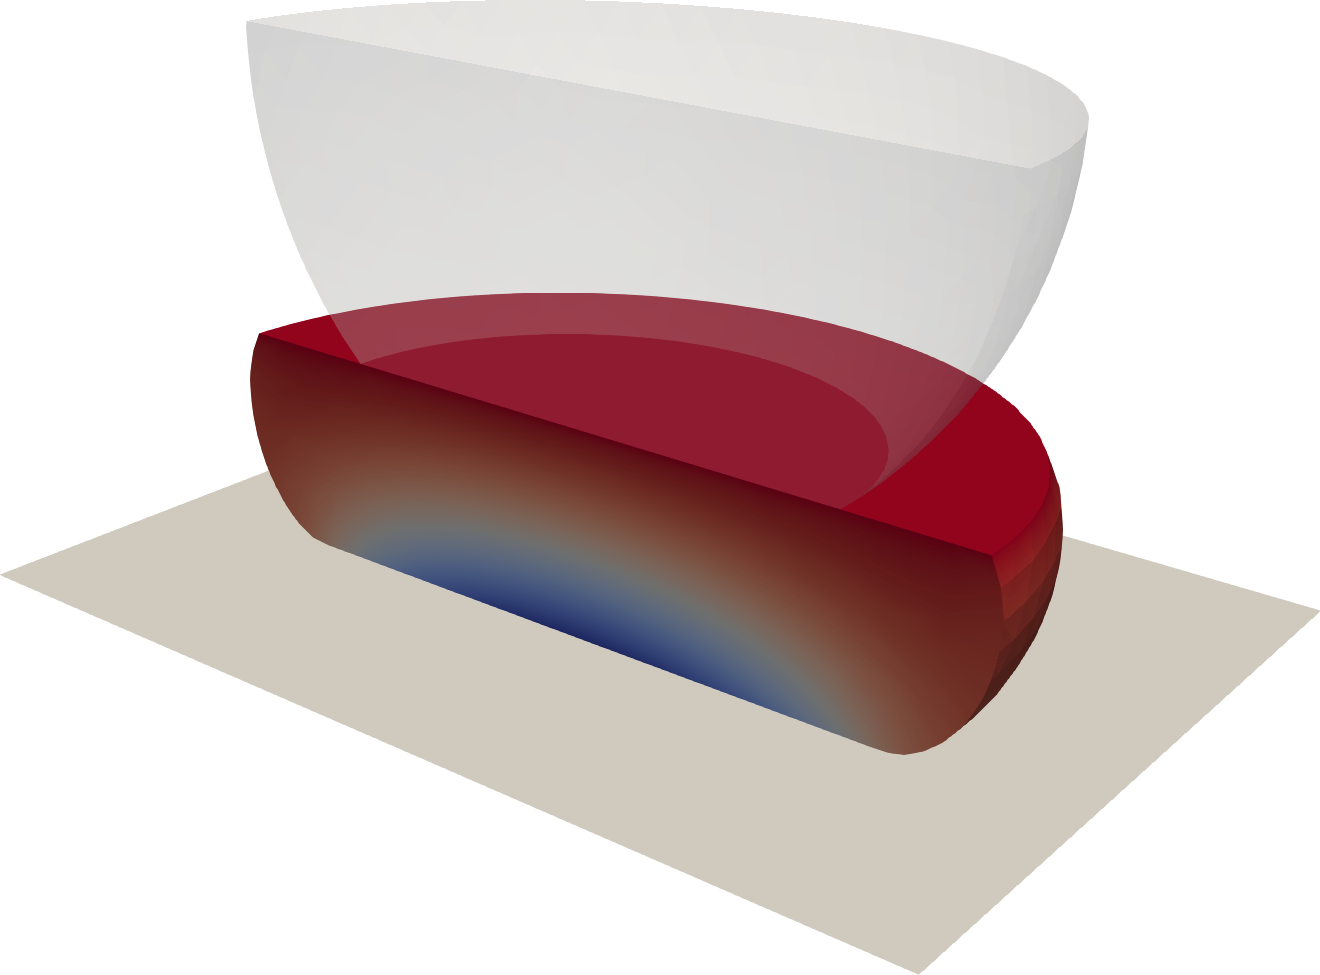
\includegraphics[width=0.7\linewidth]{figures/redo.png}}
    \end{subcaptionbox}    \hfill
%    \vspace{0.5cm} % Adjust vertical spacing
    \begin{subcaptionbox}{$K = \{ |\nabla u| \le \phi\}$}[0.3\textwidth]
        {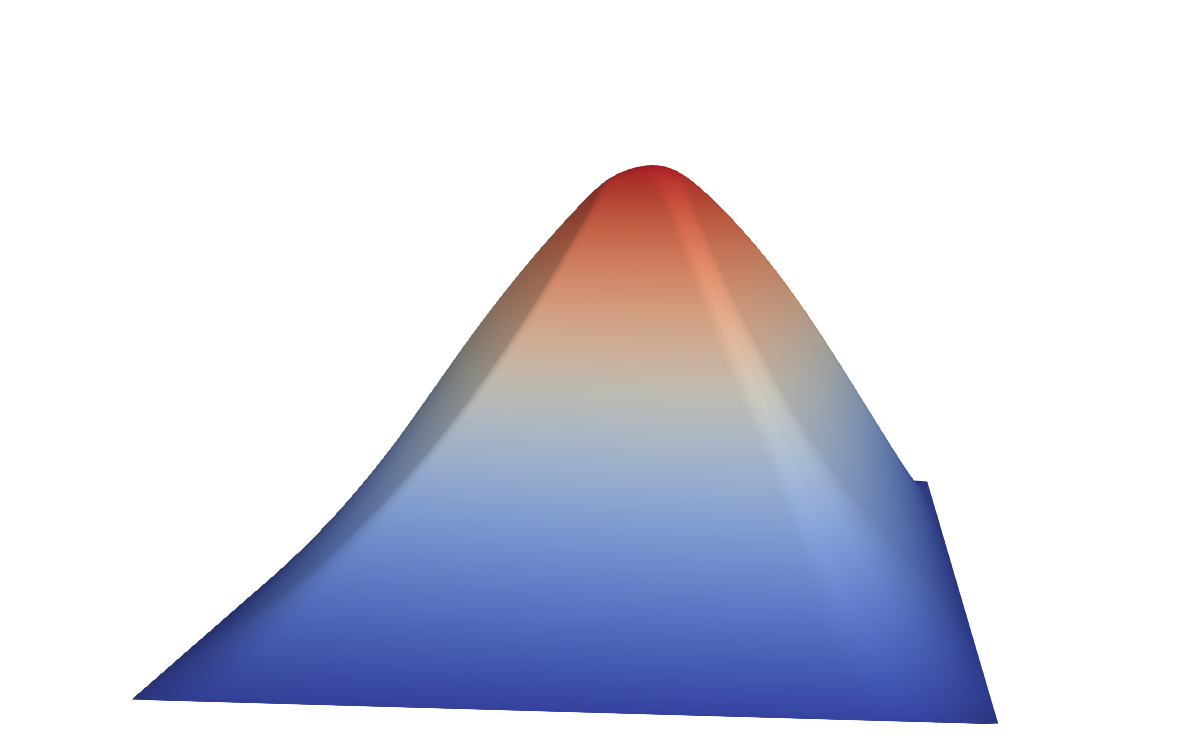
\includegraphics[width=0.7\linewidth]{figures/gradient_constraint_u.png}}
    \end{subcaptionbox}

%    \caption{Main caption for all four figures.}
\end{figure}
%\hypertarget{lvpp-examples}{}
%\hyperlink{lvpp-table}{\beamerbutton{Go to Table}}\vspace{-2ex}
%

\begin{minipage}{0.41\linewidth}\small
$K = \left\{\sum_i u_i = 1, u_i \ge 0\right\}$: Evolution of a multiphase Cahn--Hilliard problem at several times steps $t$.
\end{minipage}%
\begin{minipage}{0.6\linewidth}
\begin{figure}
    \centering
    \subcaptionbox*{$t=0$} {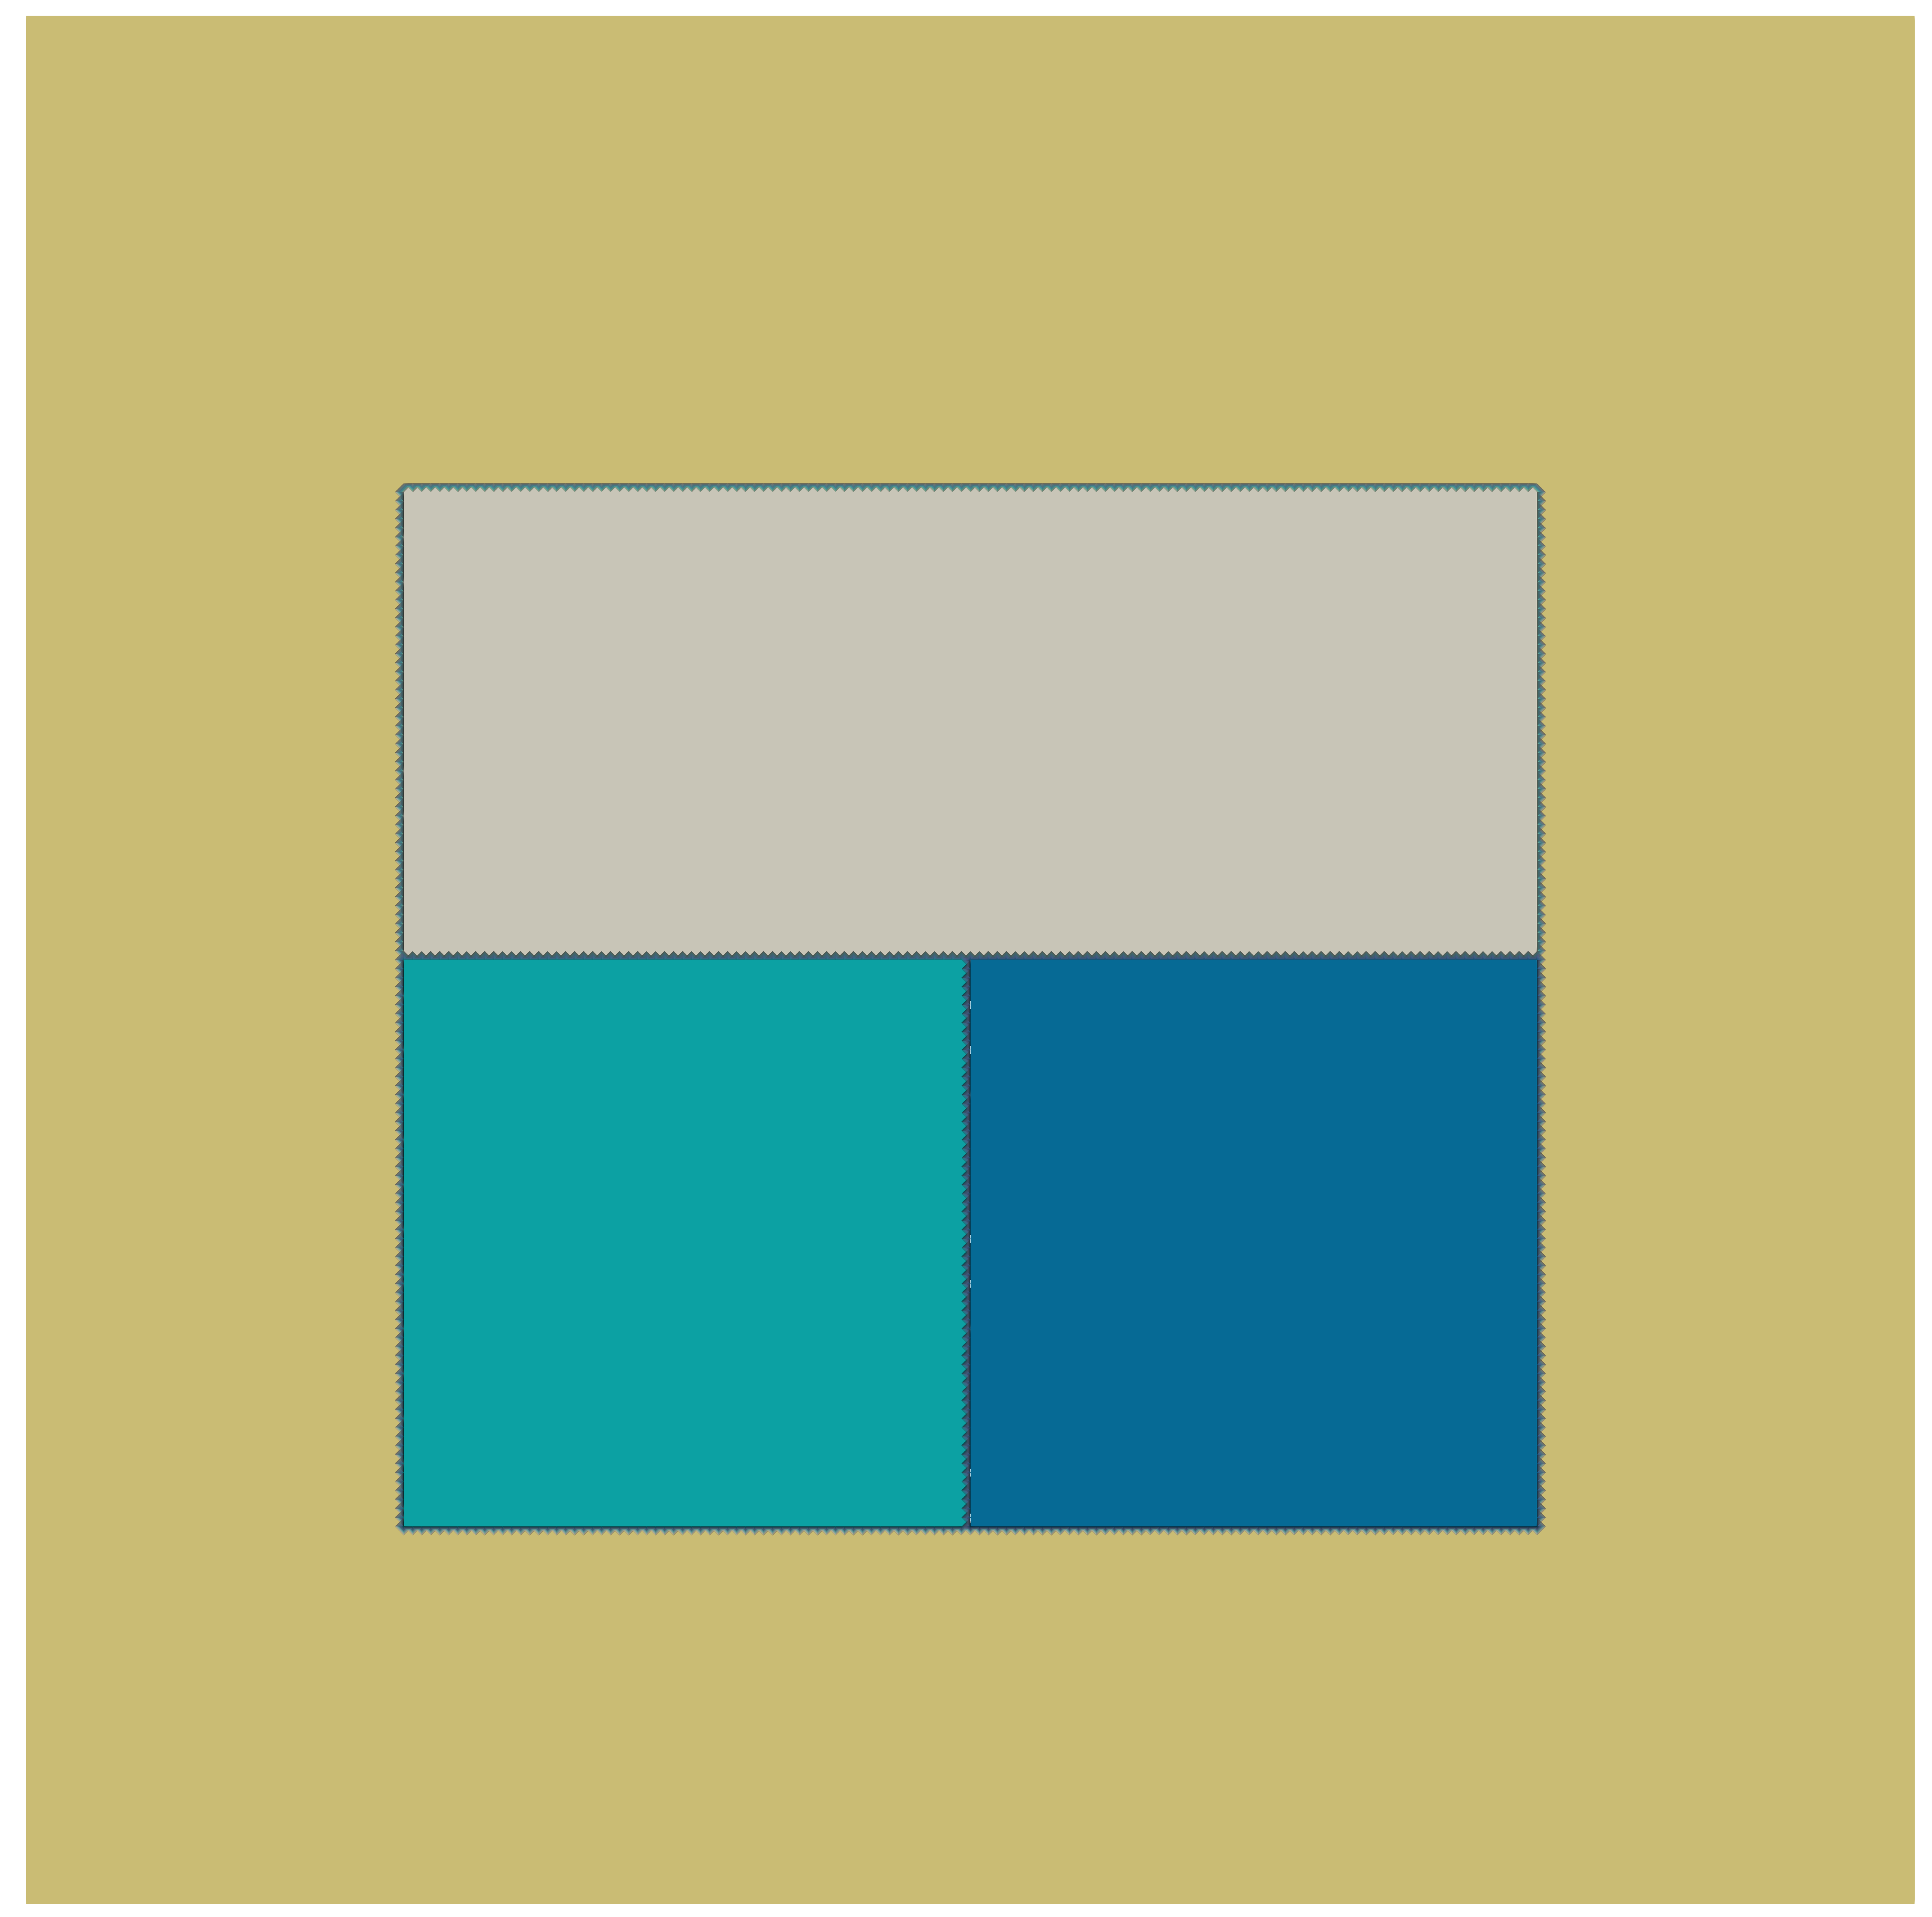
\includegraphics[width=0.23\linewidth]{figures/CH0.png}}
    \subcaptionbox*{$t=10^{-4}$} {
\includegraphics[width=0.23\linewidth]{figures/CH10.png}}
    \subcaptionbox*{$t=10^{-3}$} {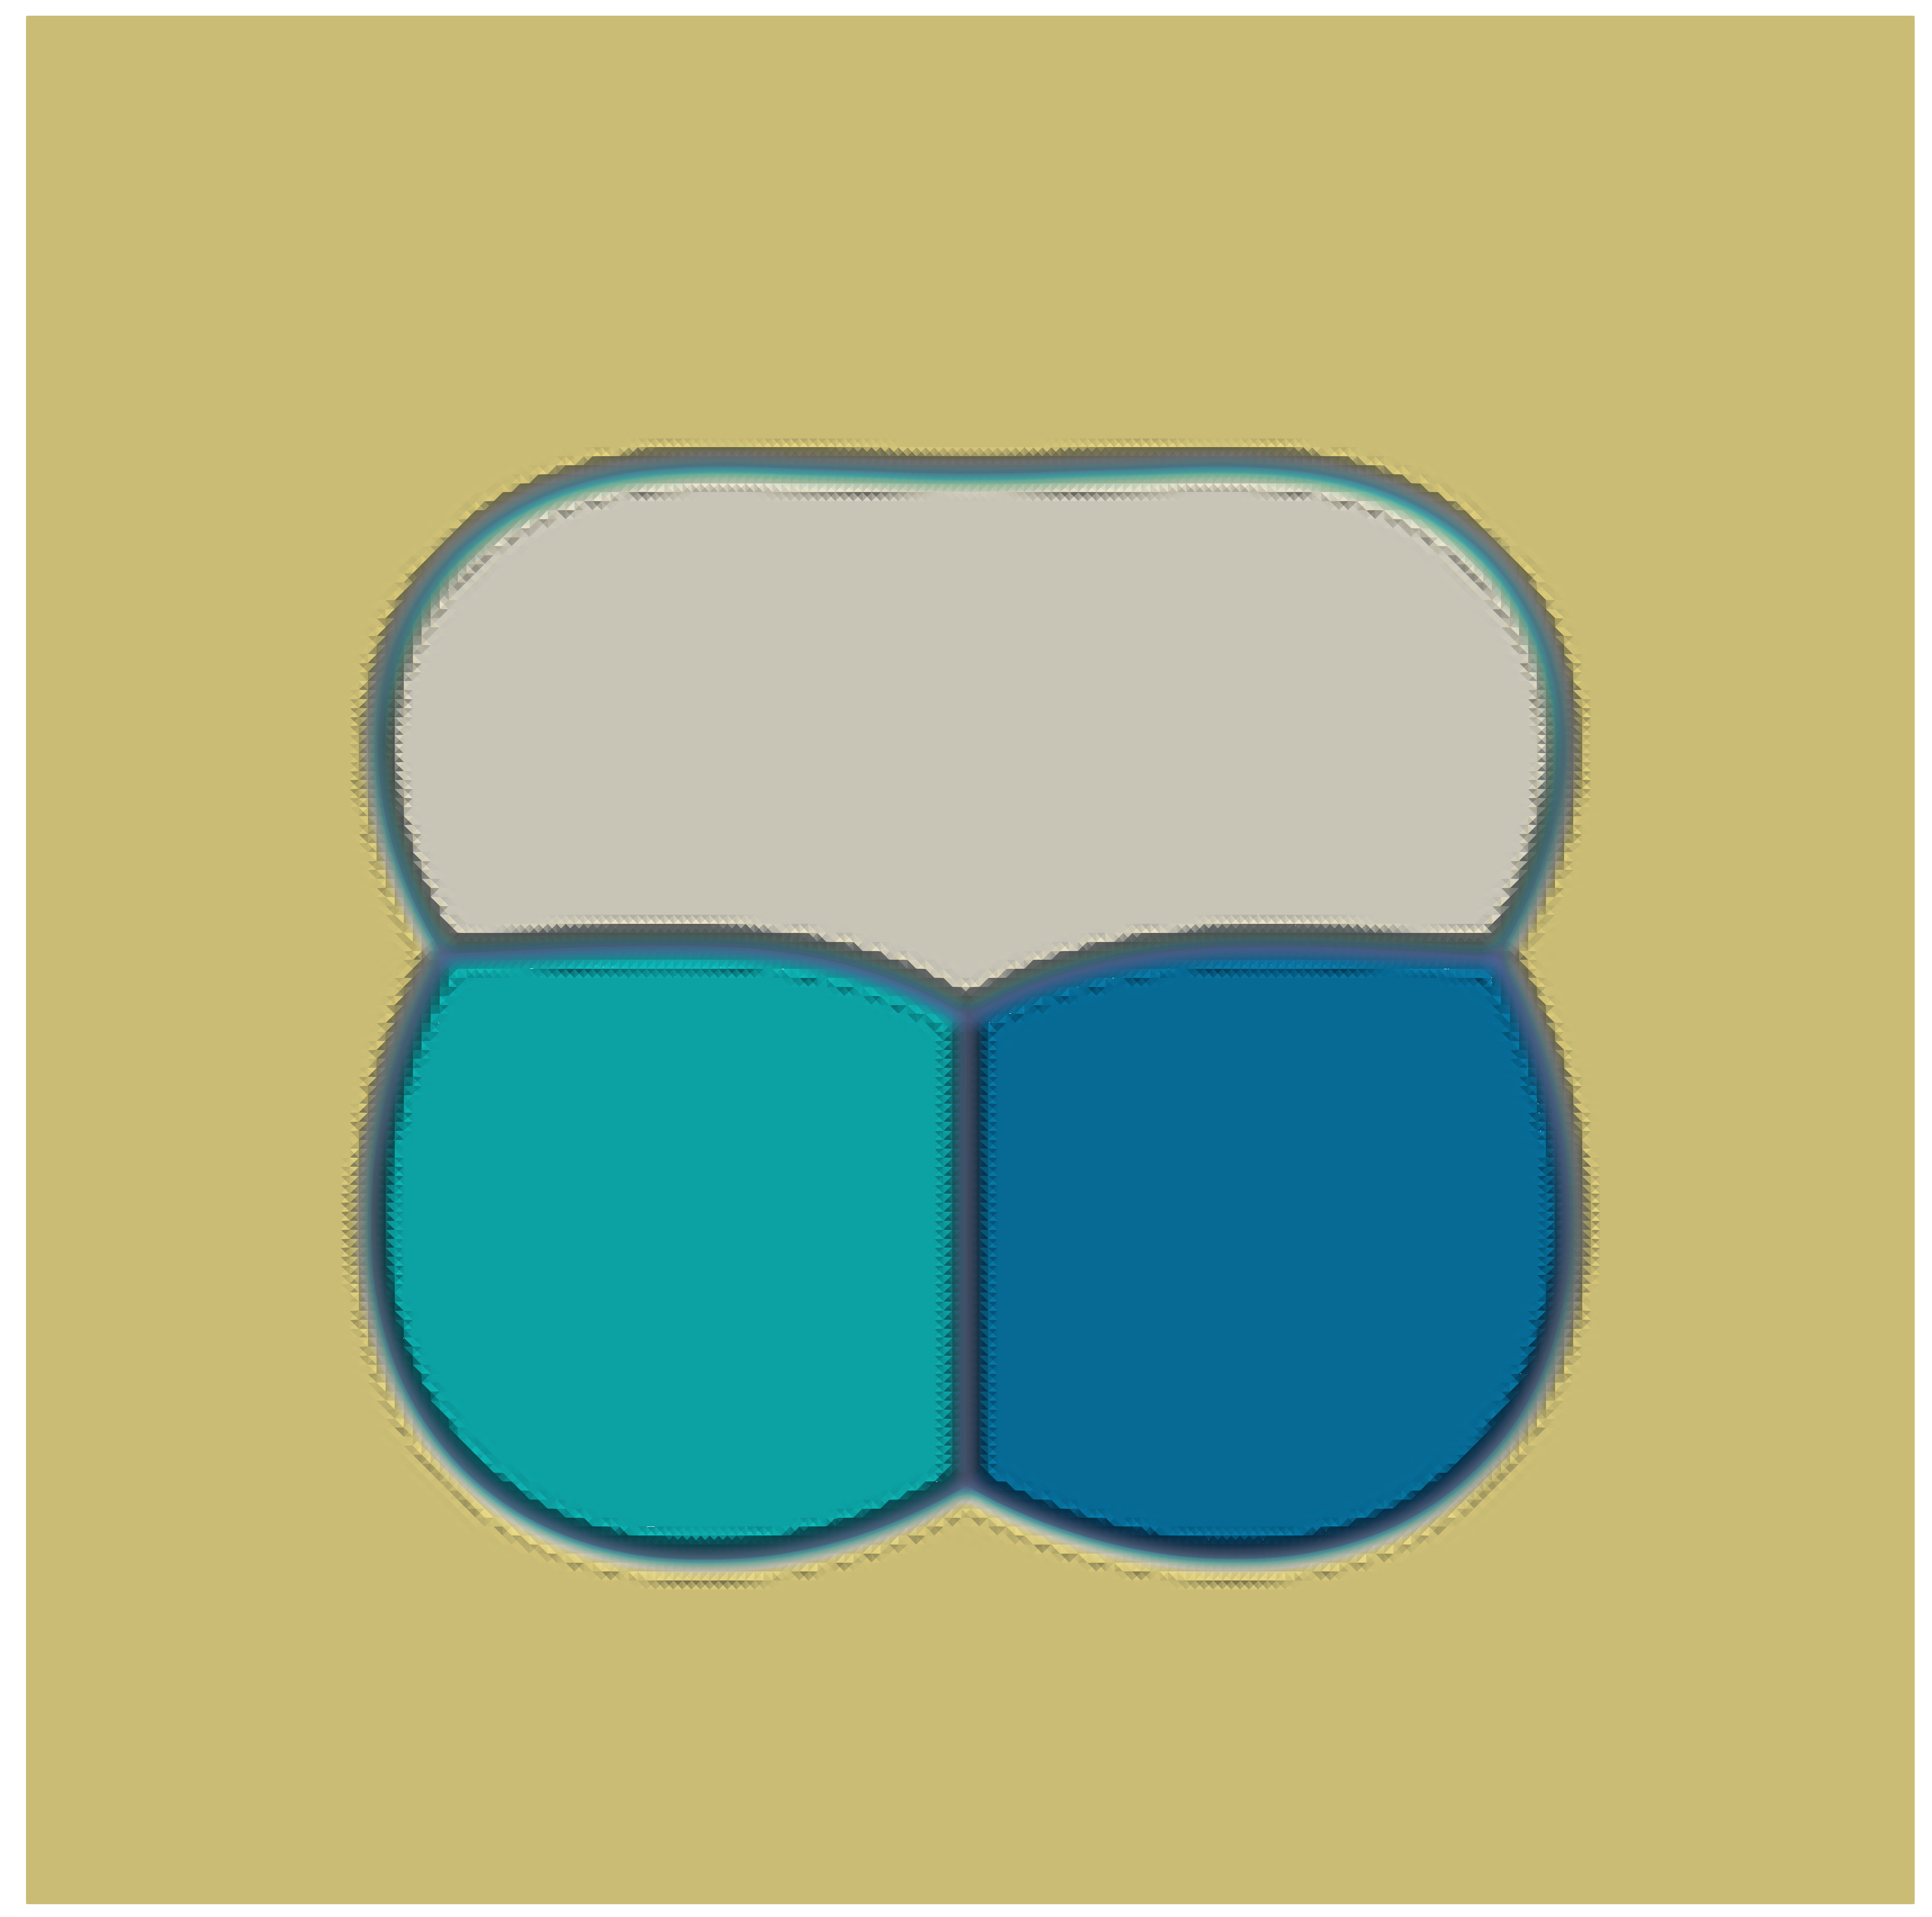
\includegraphics[width=0.23\linewidth]{figures/CH100.png}}
    \subcaptionbox*{$t=7\times 10^{-3}$} {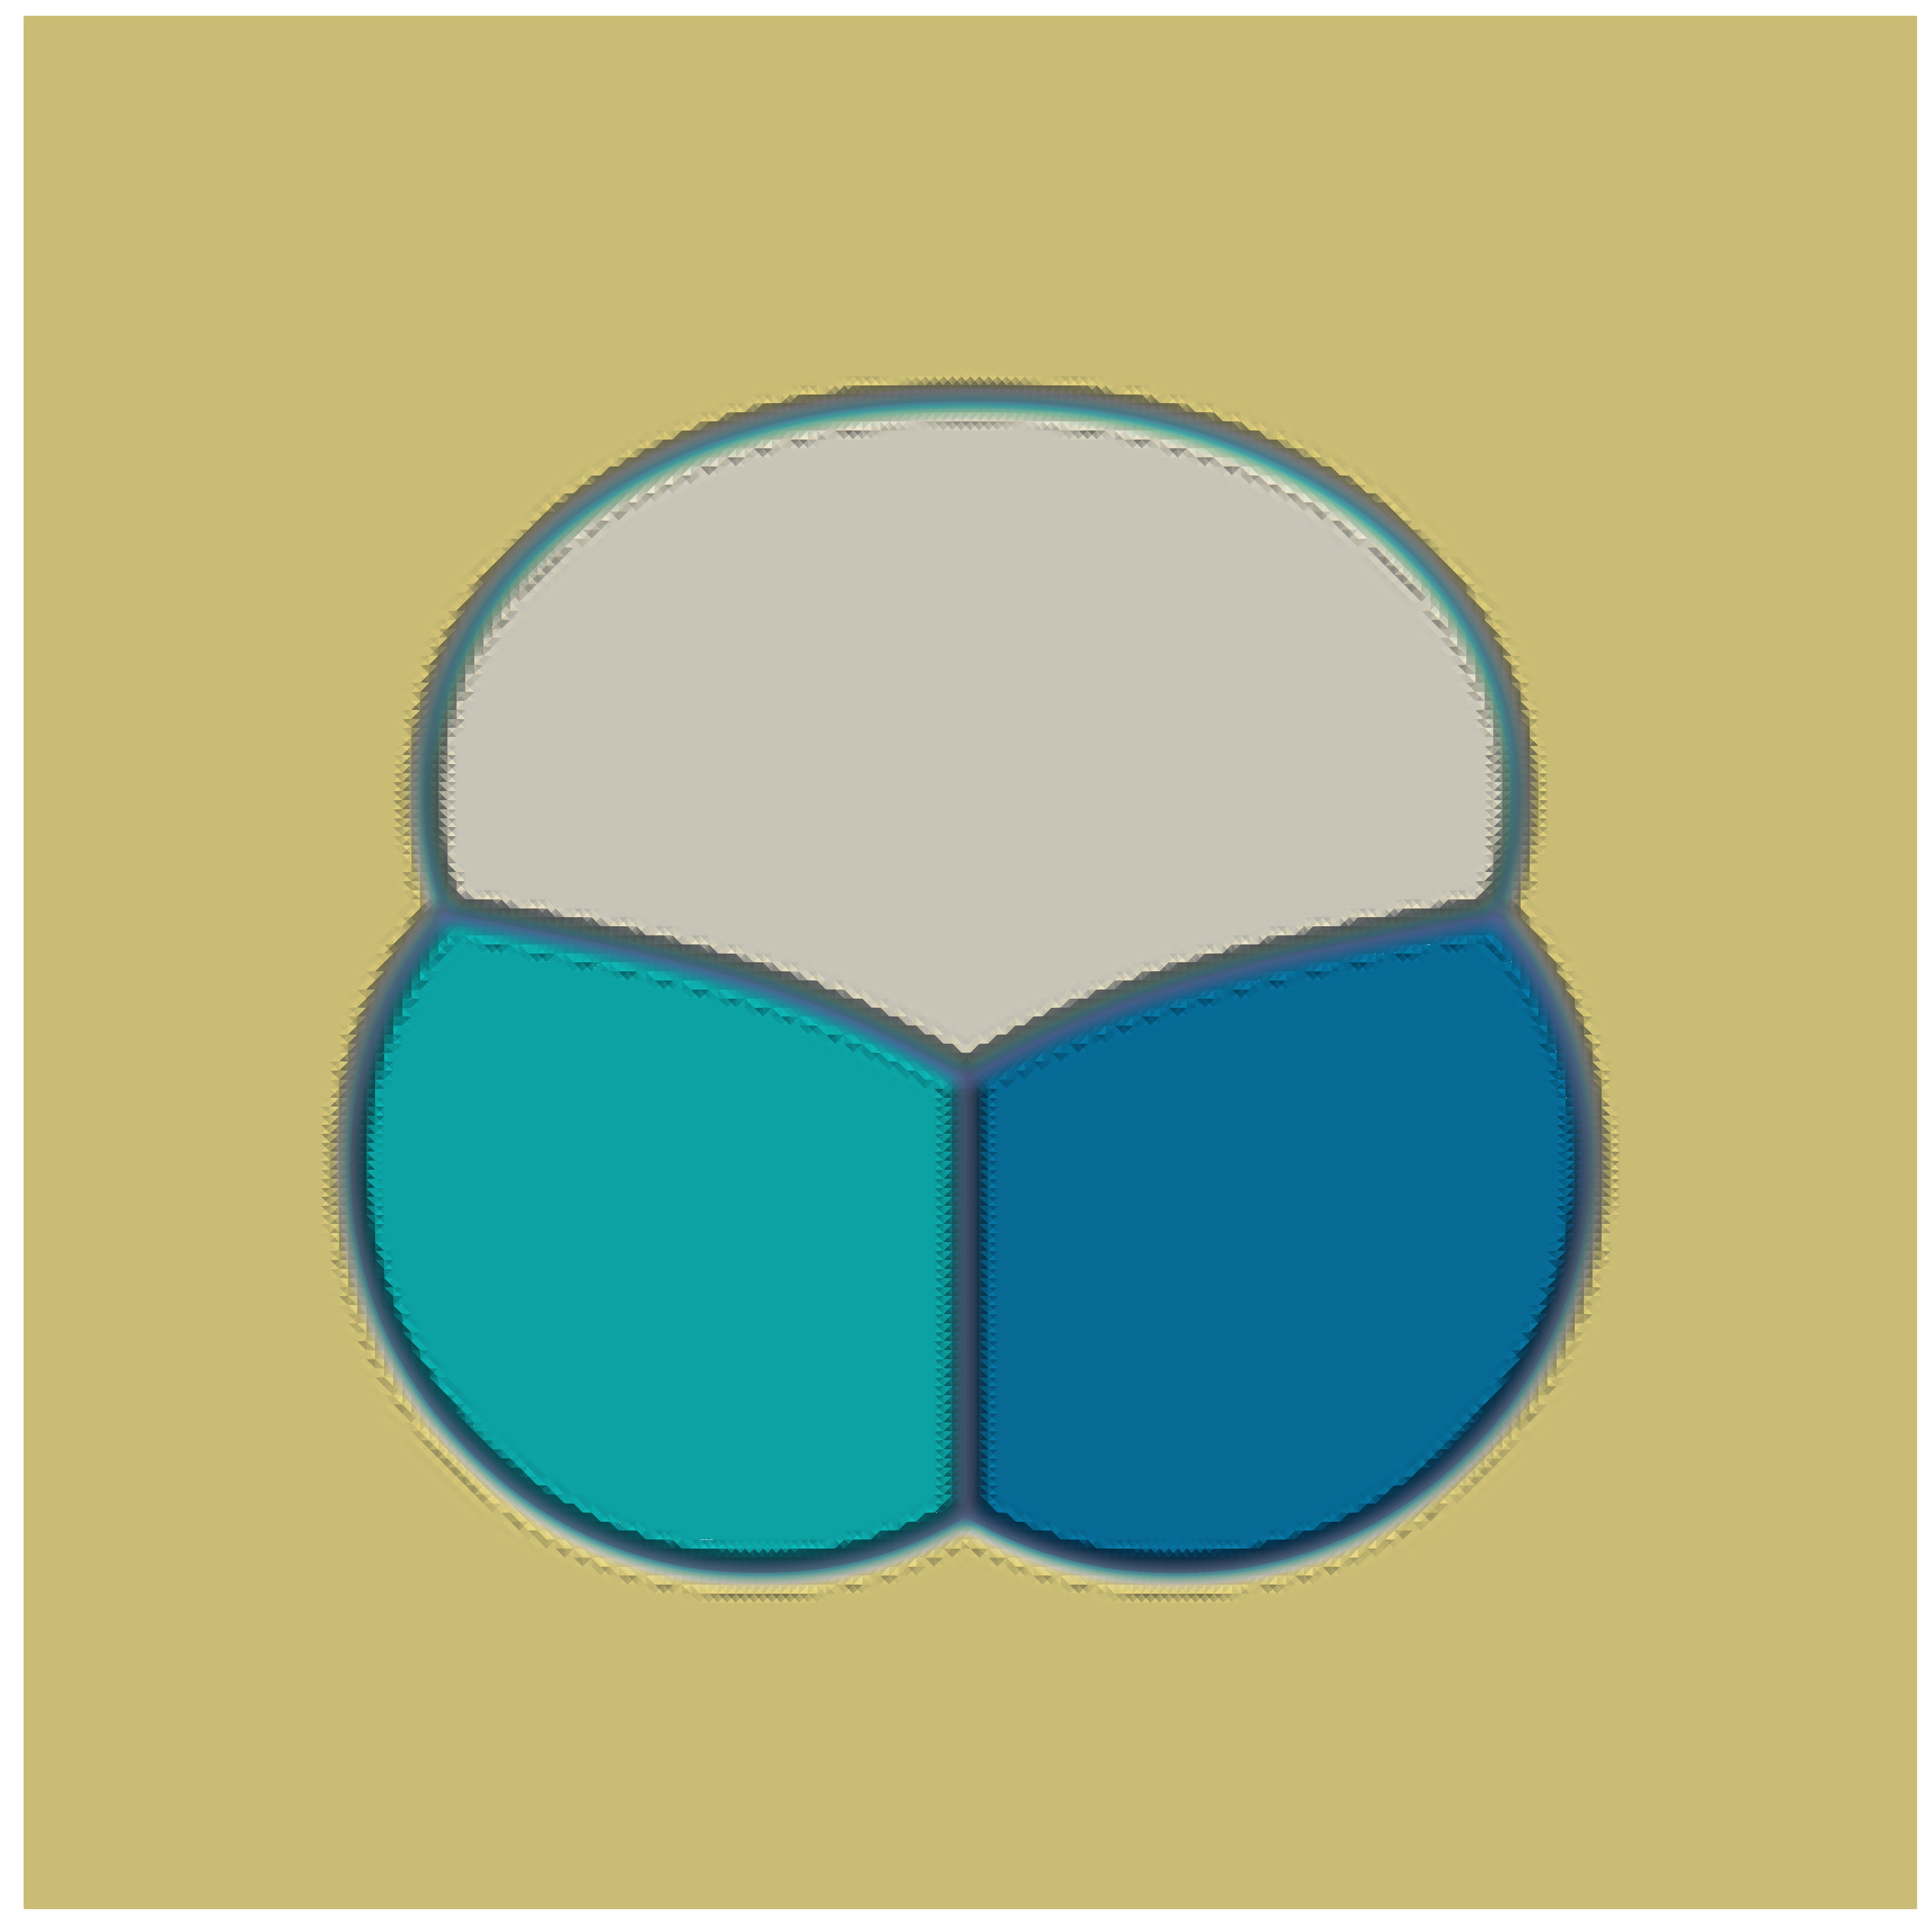
\includegraphics[width=0.23\linewidth]{figures/CH700.png}}\vspace{-2ex}
%    % \includegraphics[width=0.30\linewidth]{Figures/species_0.25.png}
%    % \includegraphics[width=0.30\linewidth]{Figures/species_0.5.png}
%    \caption{\footnotesize}
    % $t=0, 10^{-4}$, $10^{-3}$, $7\times10^{-3}$.}
    \label{fig:cahn-hilliard}
\end{figure}\vspace{-2ex}
\end{minipage}

\end{frame}

\begin{frame}{Other Potential Applications}
\begin{figure}
  \centering
  \begin{subfigure}[b]{0.19\textwidth}
    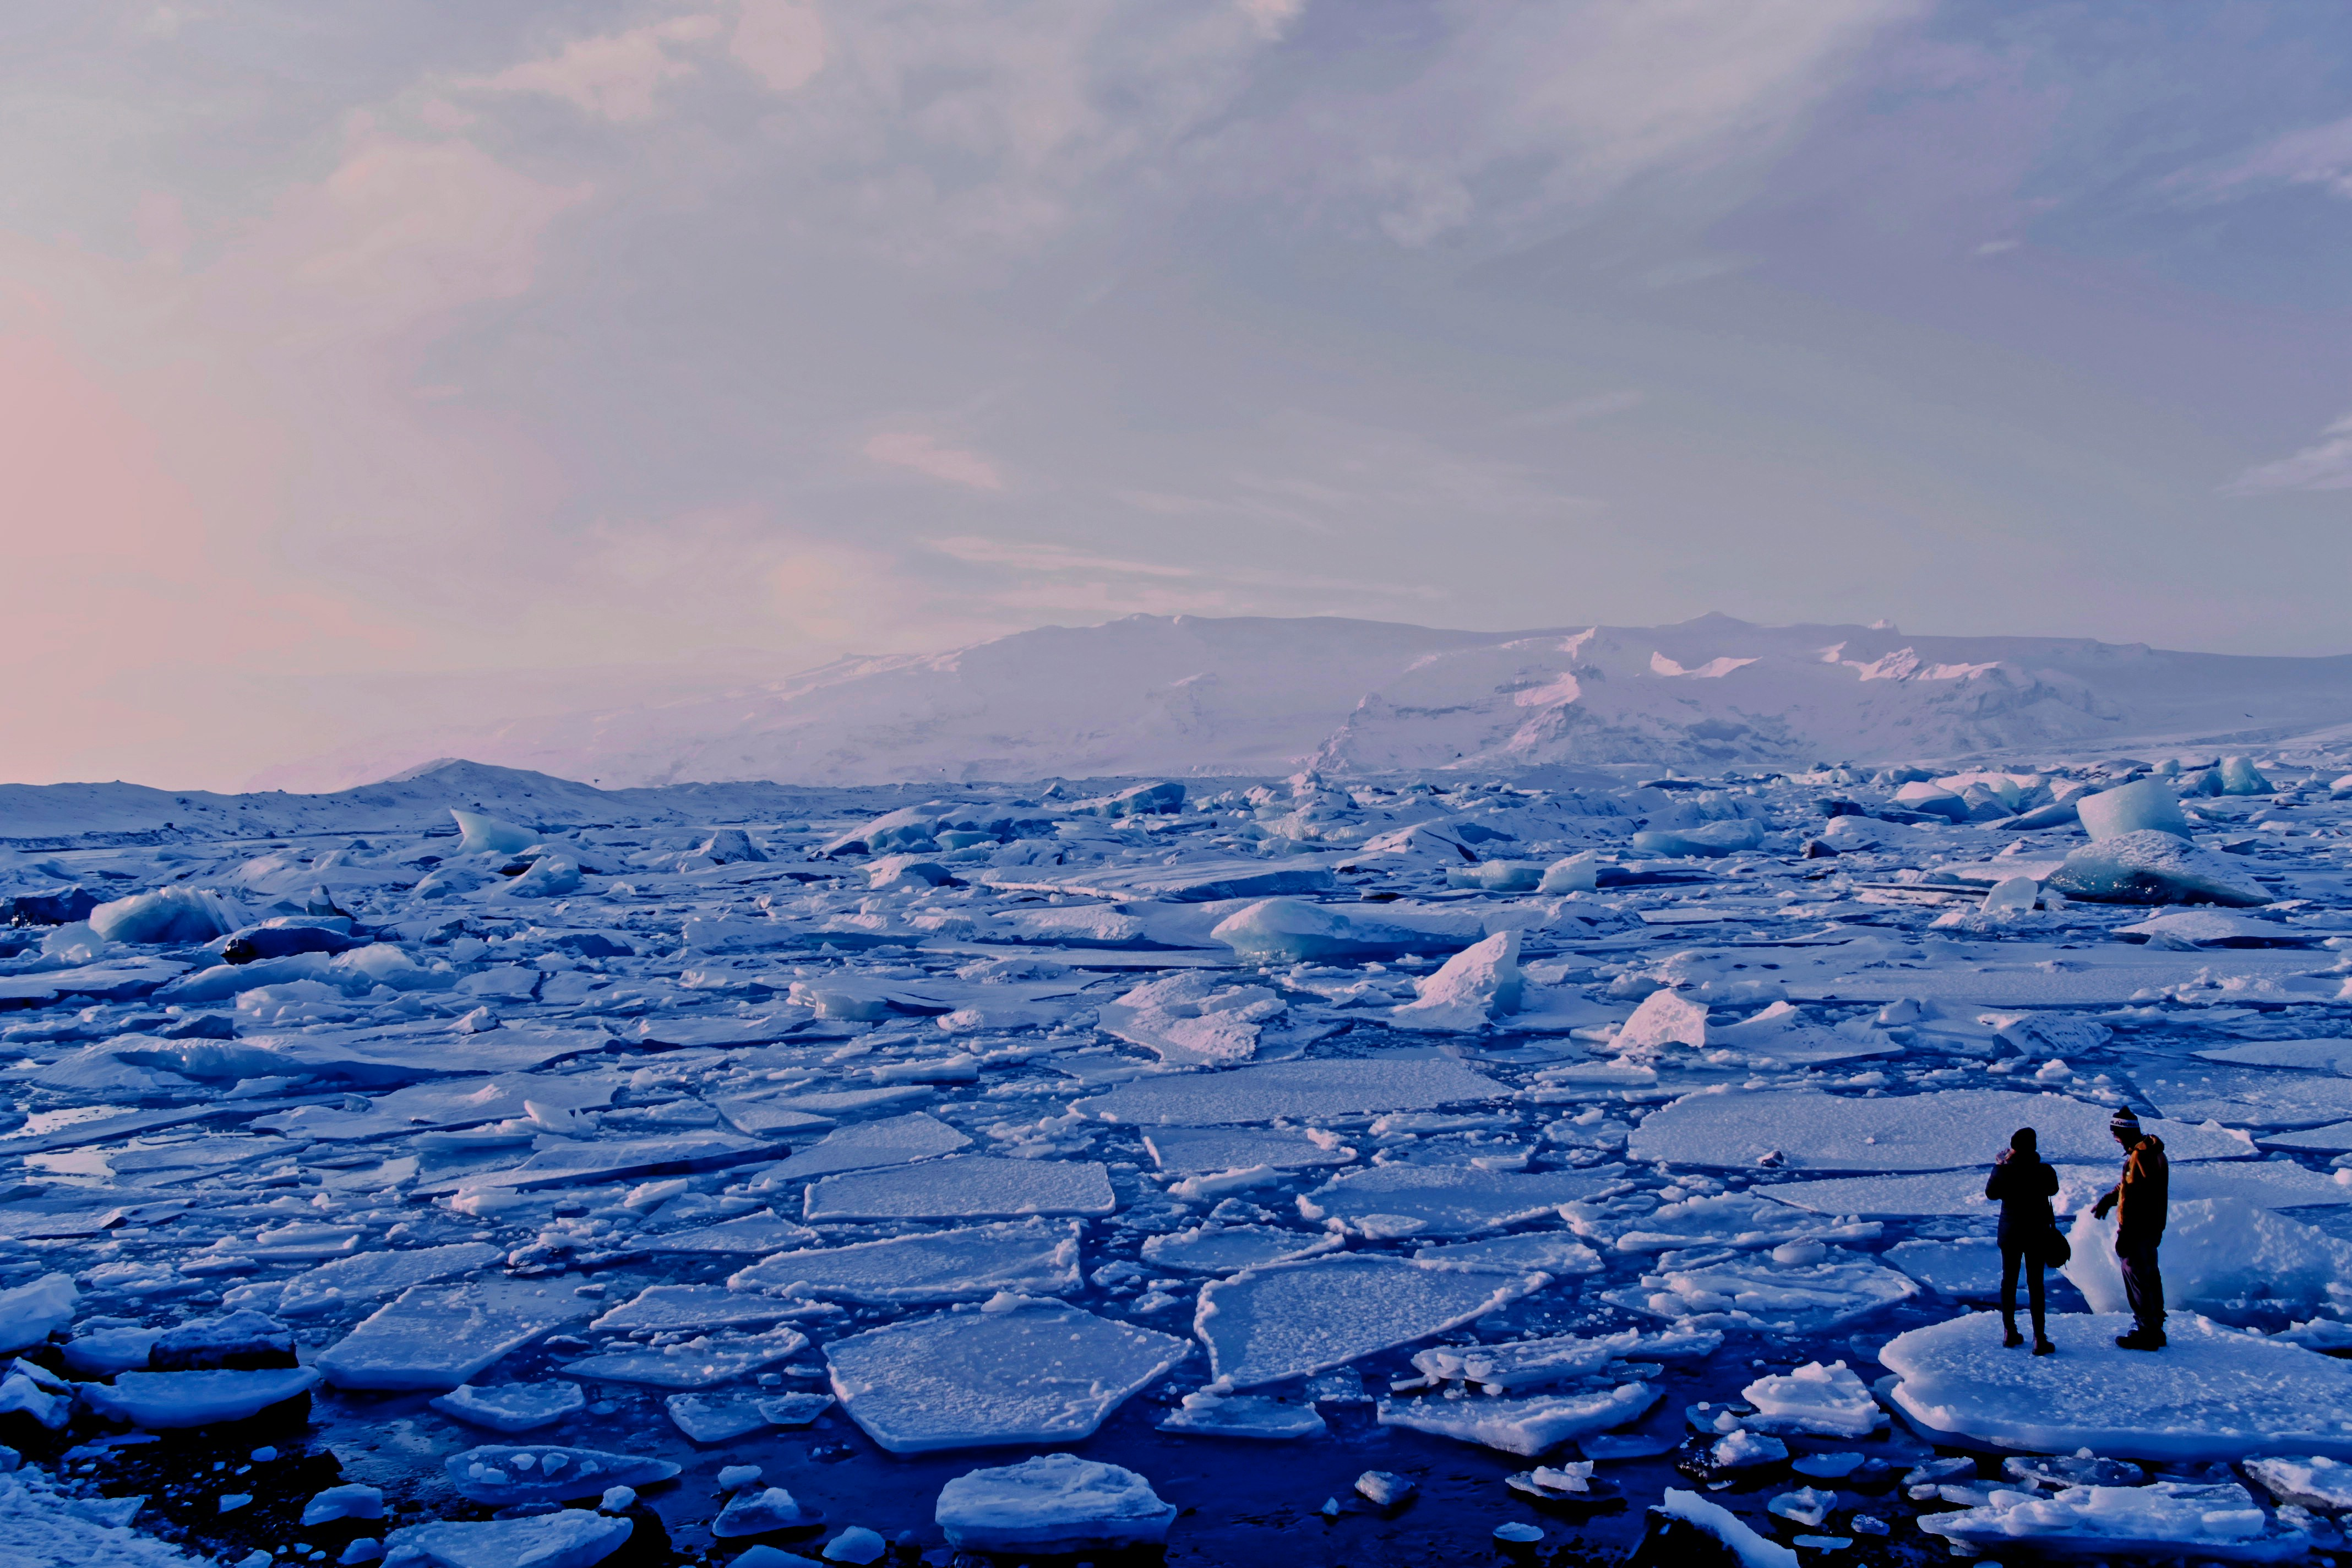
\includegraphics[width=\linewidth]{figures/ice.jpg}
    \caption{Stefan Problem}
  \end{subfigure}
  \hfill
  \begin{subfigure}[b]{0.19\textwidth}
    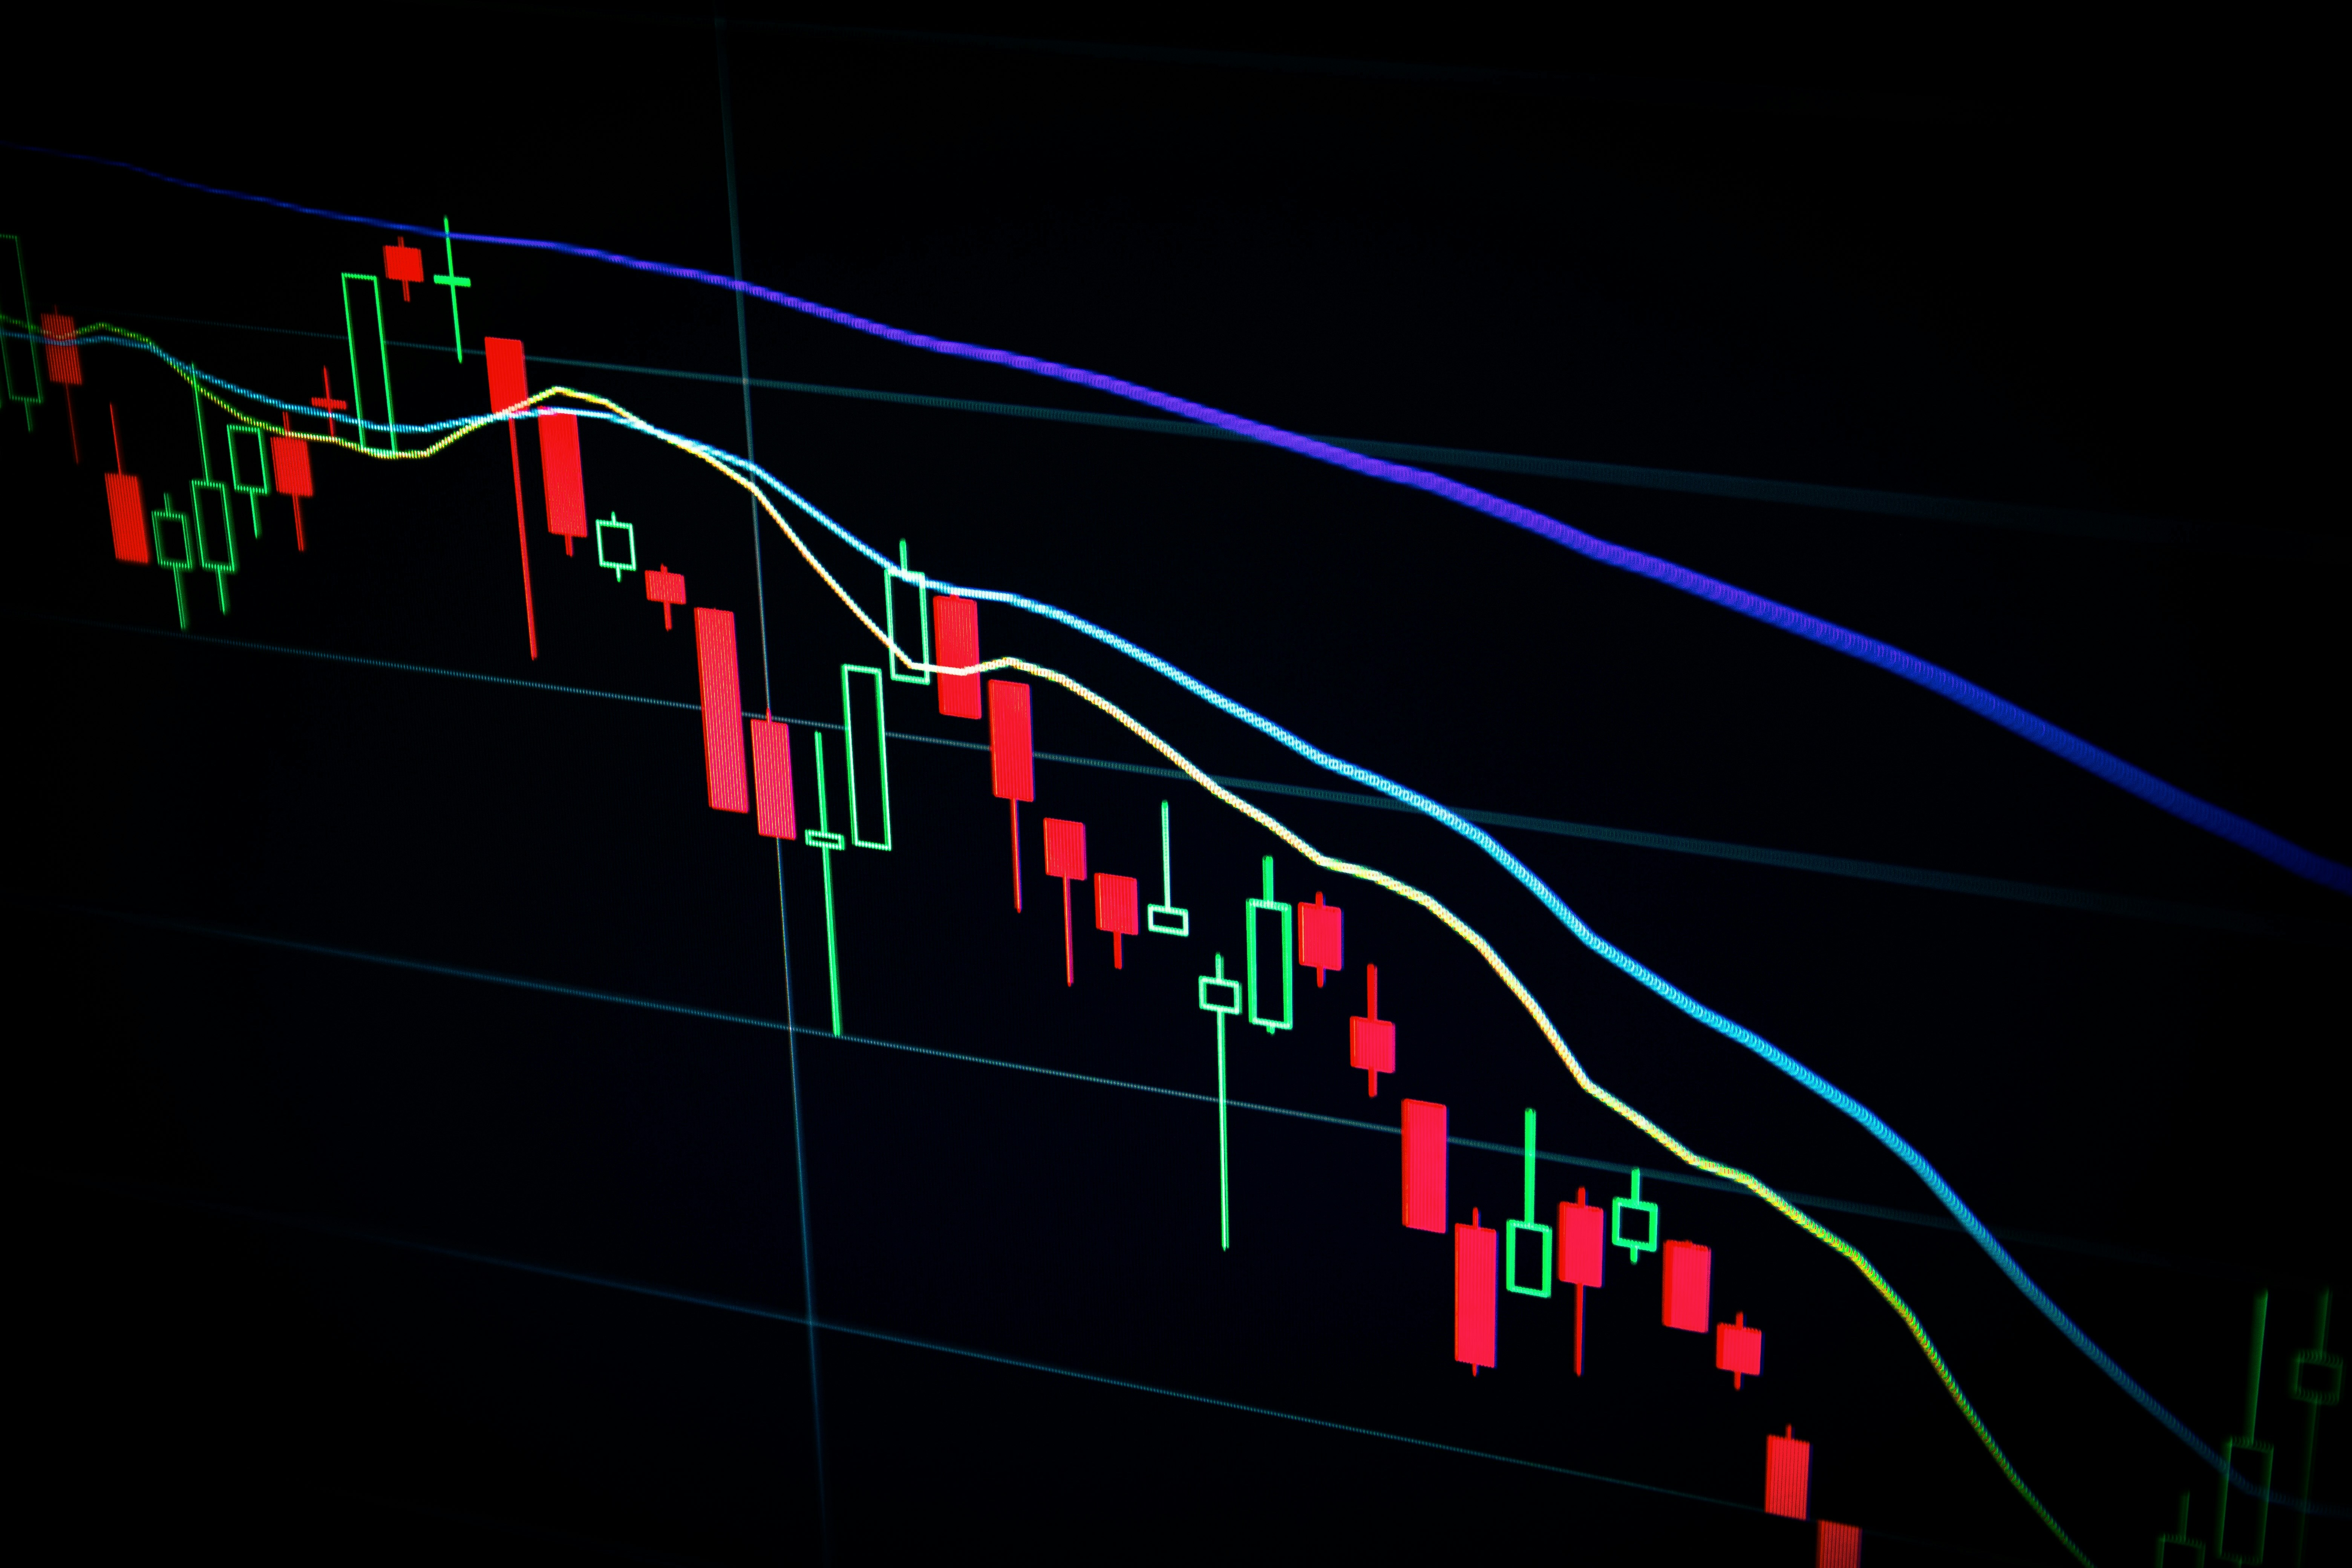
\includegraphics[width=\linewidth]{figures/stocks.jpg}
    \caption{Option Pricing}
  \end{subfigure}
  \hfill
  \begin{subfigure}[b]{0.19\textwidth}
    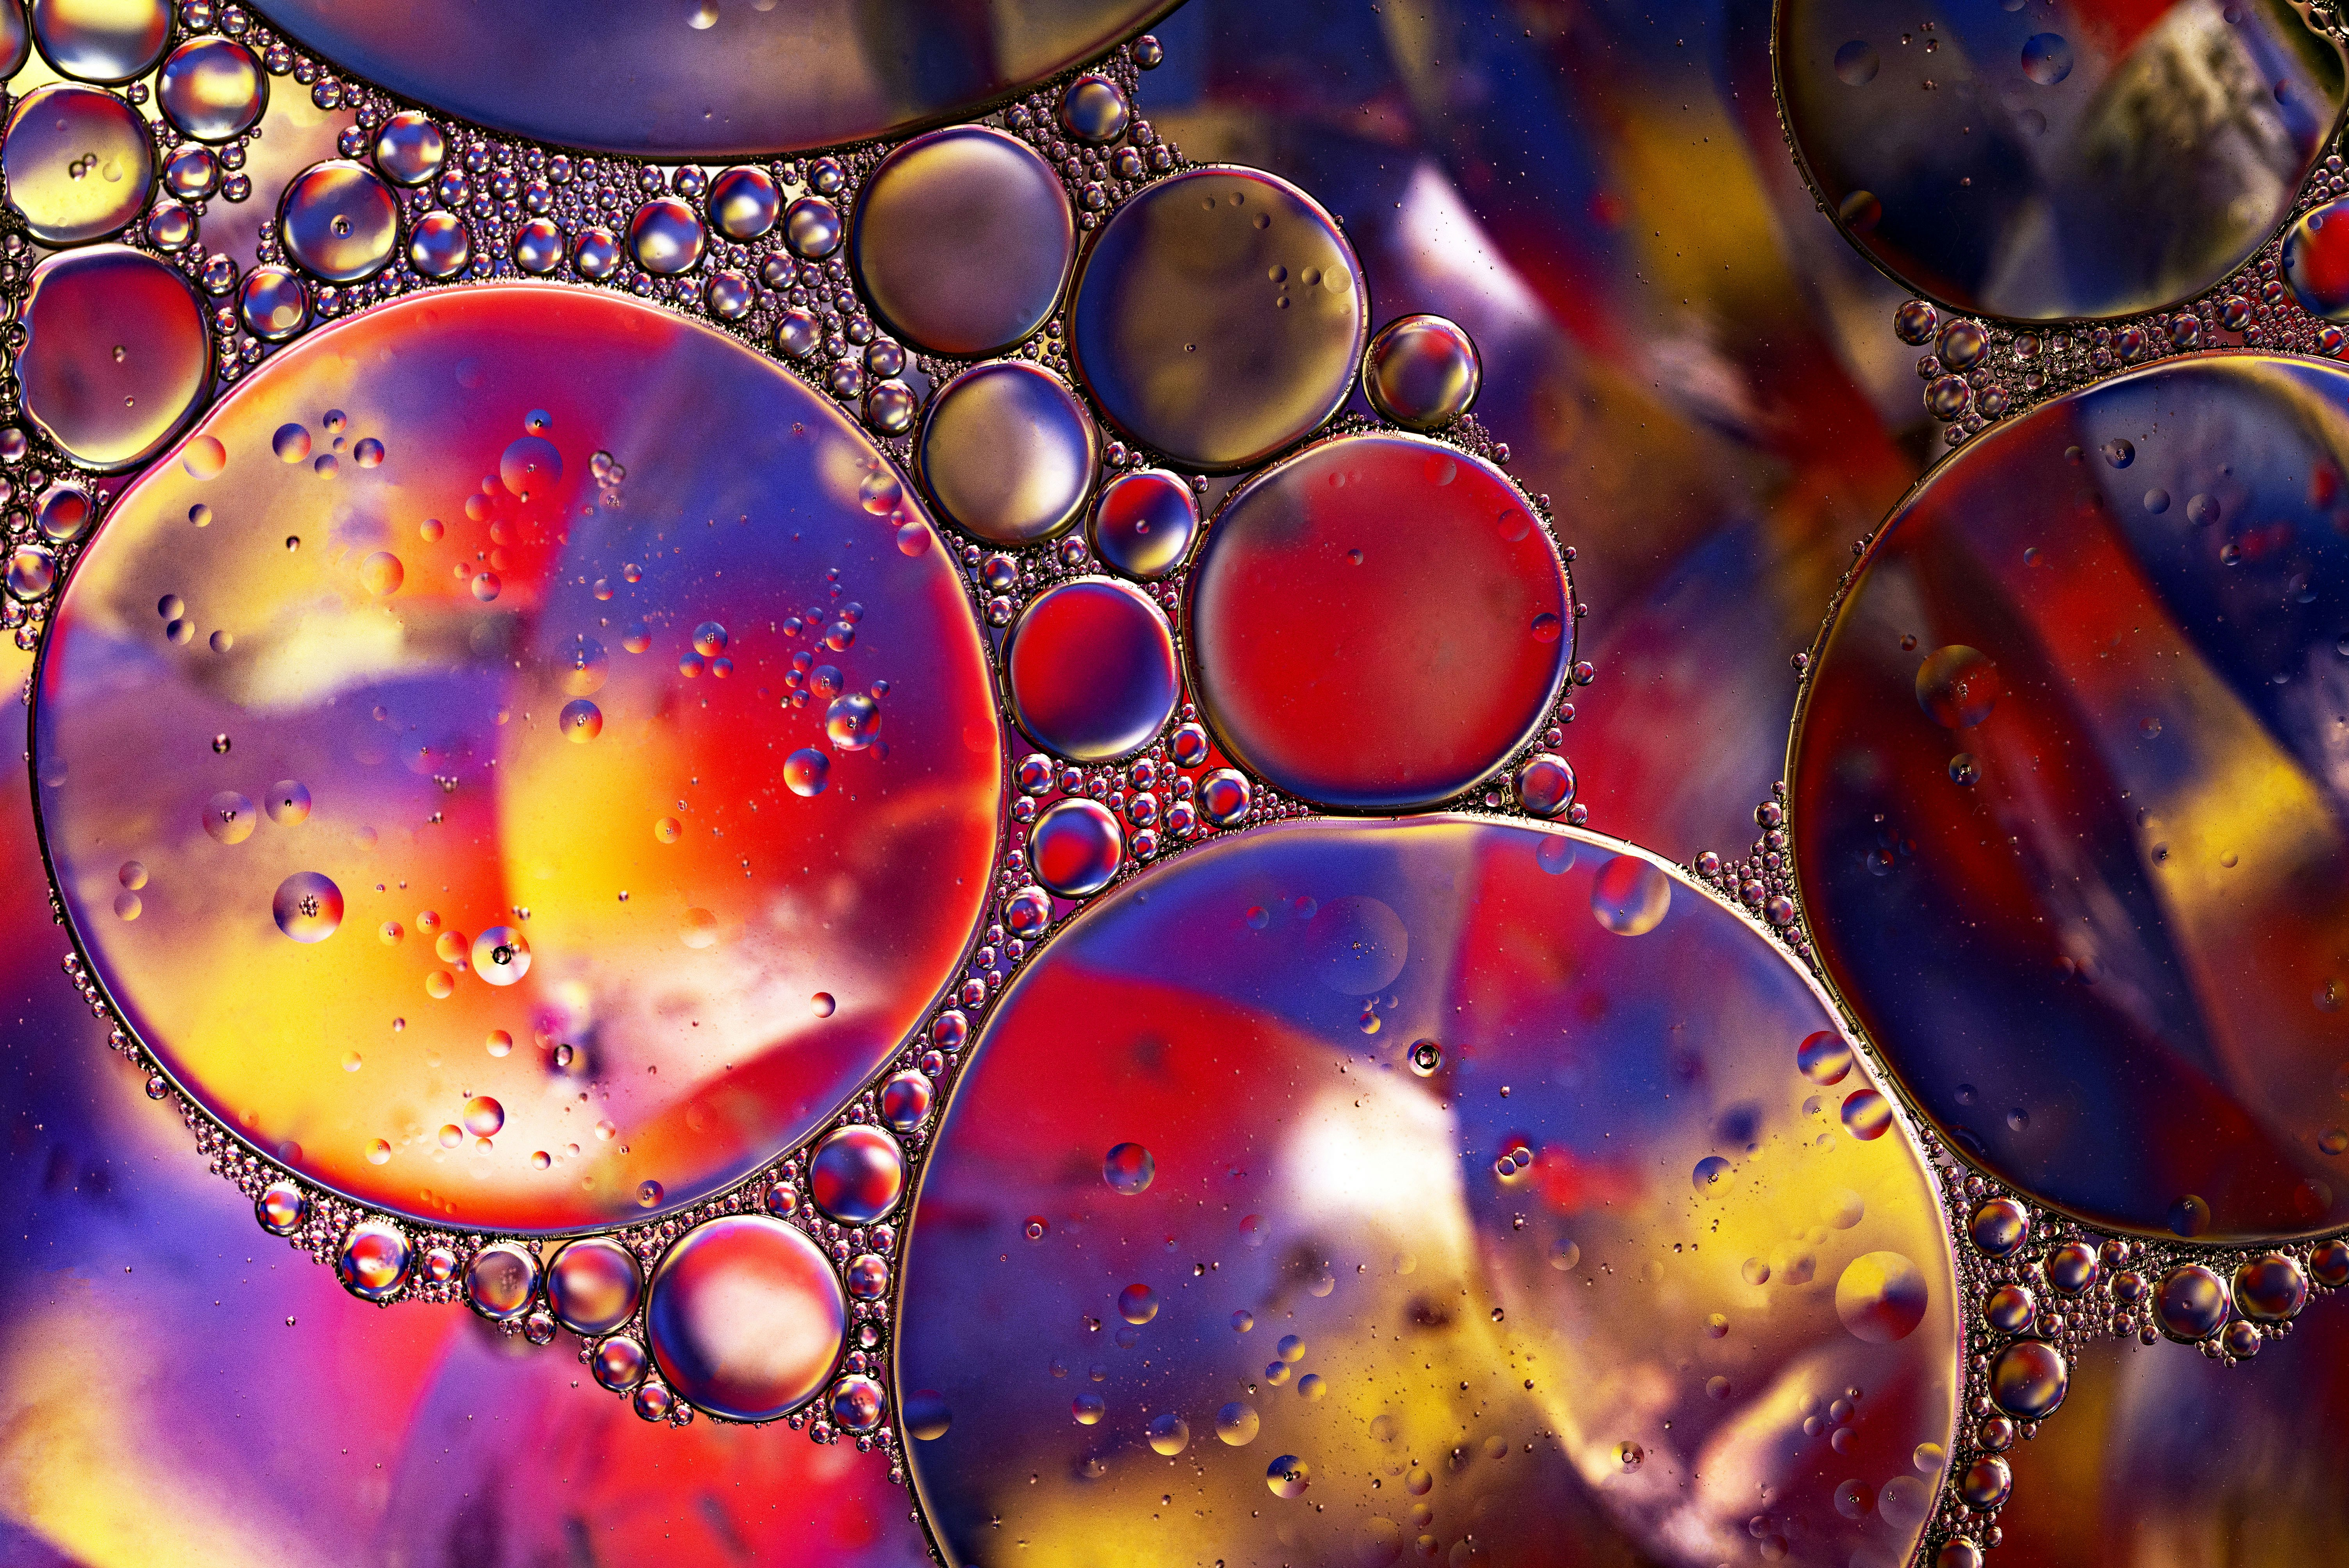
\includegraphics[width=\linewidth]{figures/water-oil-2.jpg}
    \caption{Phase Transition}
  \end{subfigure}\\
%  \hfill
  \begin{subfigure}[b]{0.19\textwidth}
    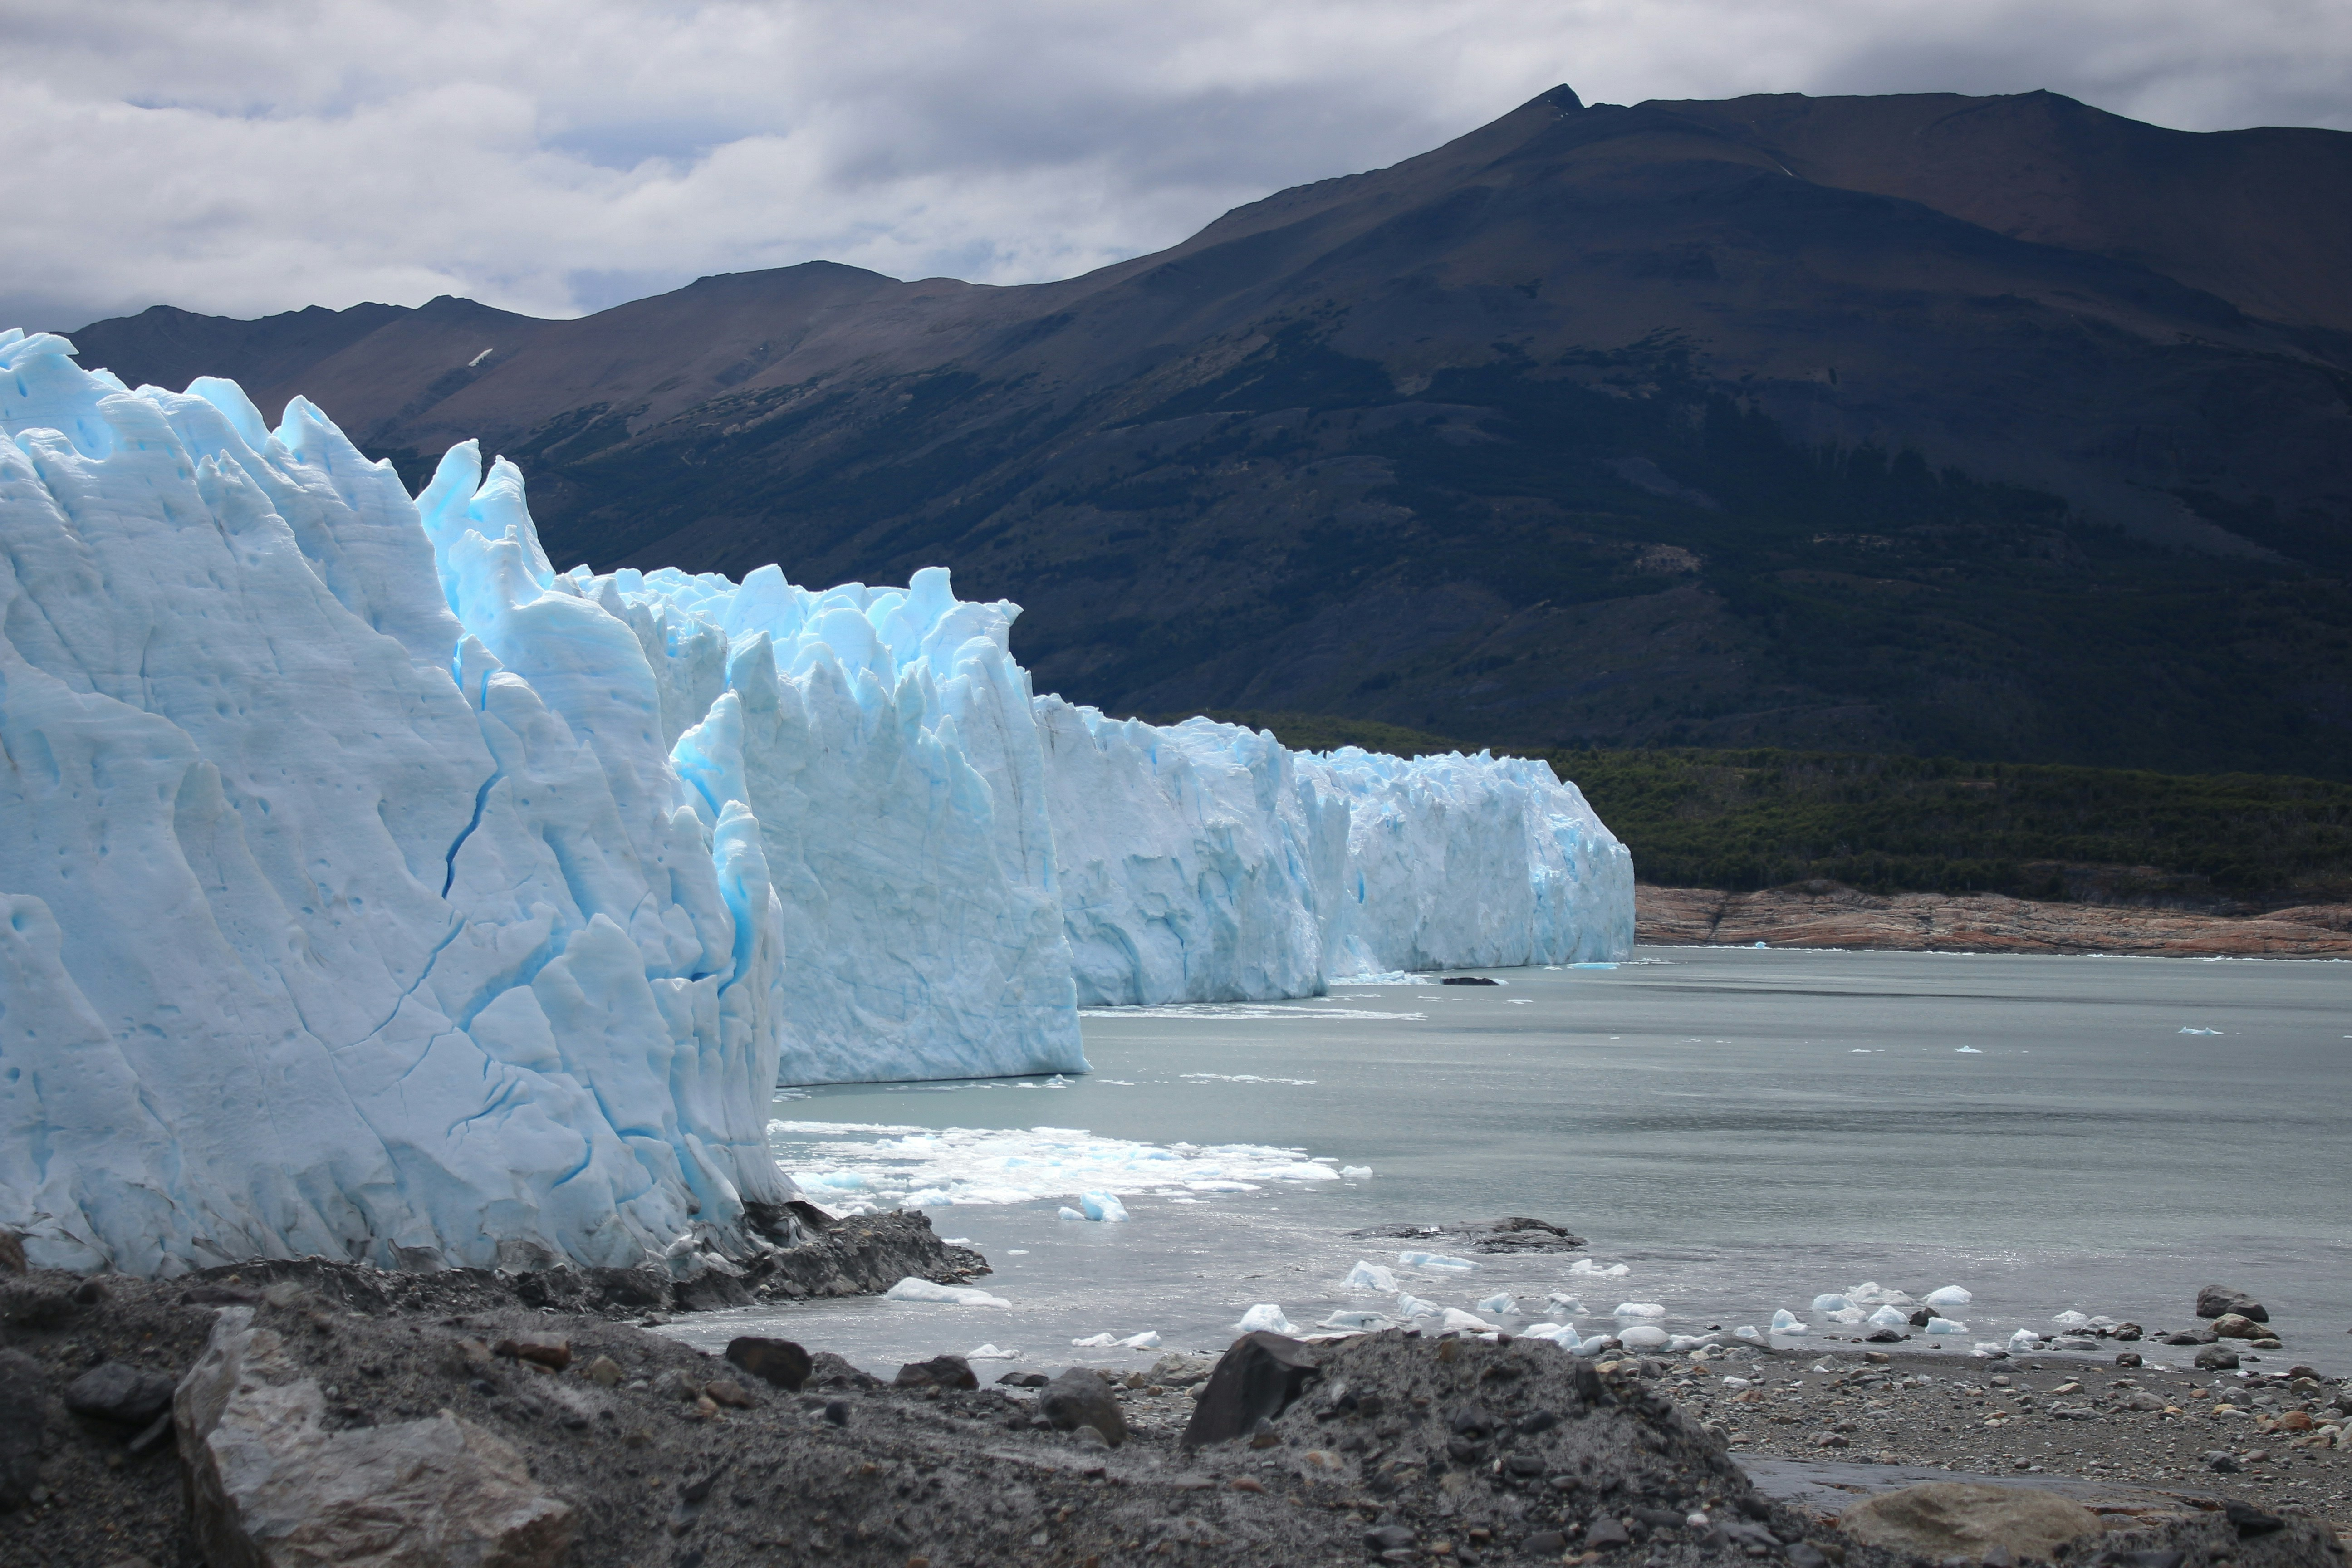
\includegraphics[width=\linewidth]{figures/glacier.jpg}
    \caption{Ice Sheet Models}
  \end{subfigure}
\hspace{7em}	
%  \hfill
  \begin{subfigure}[b]{0.19\textwidth}
    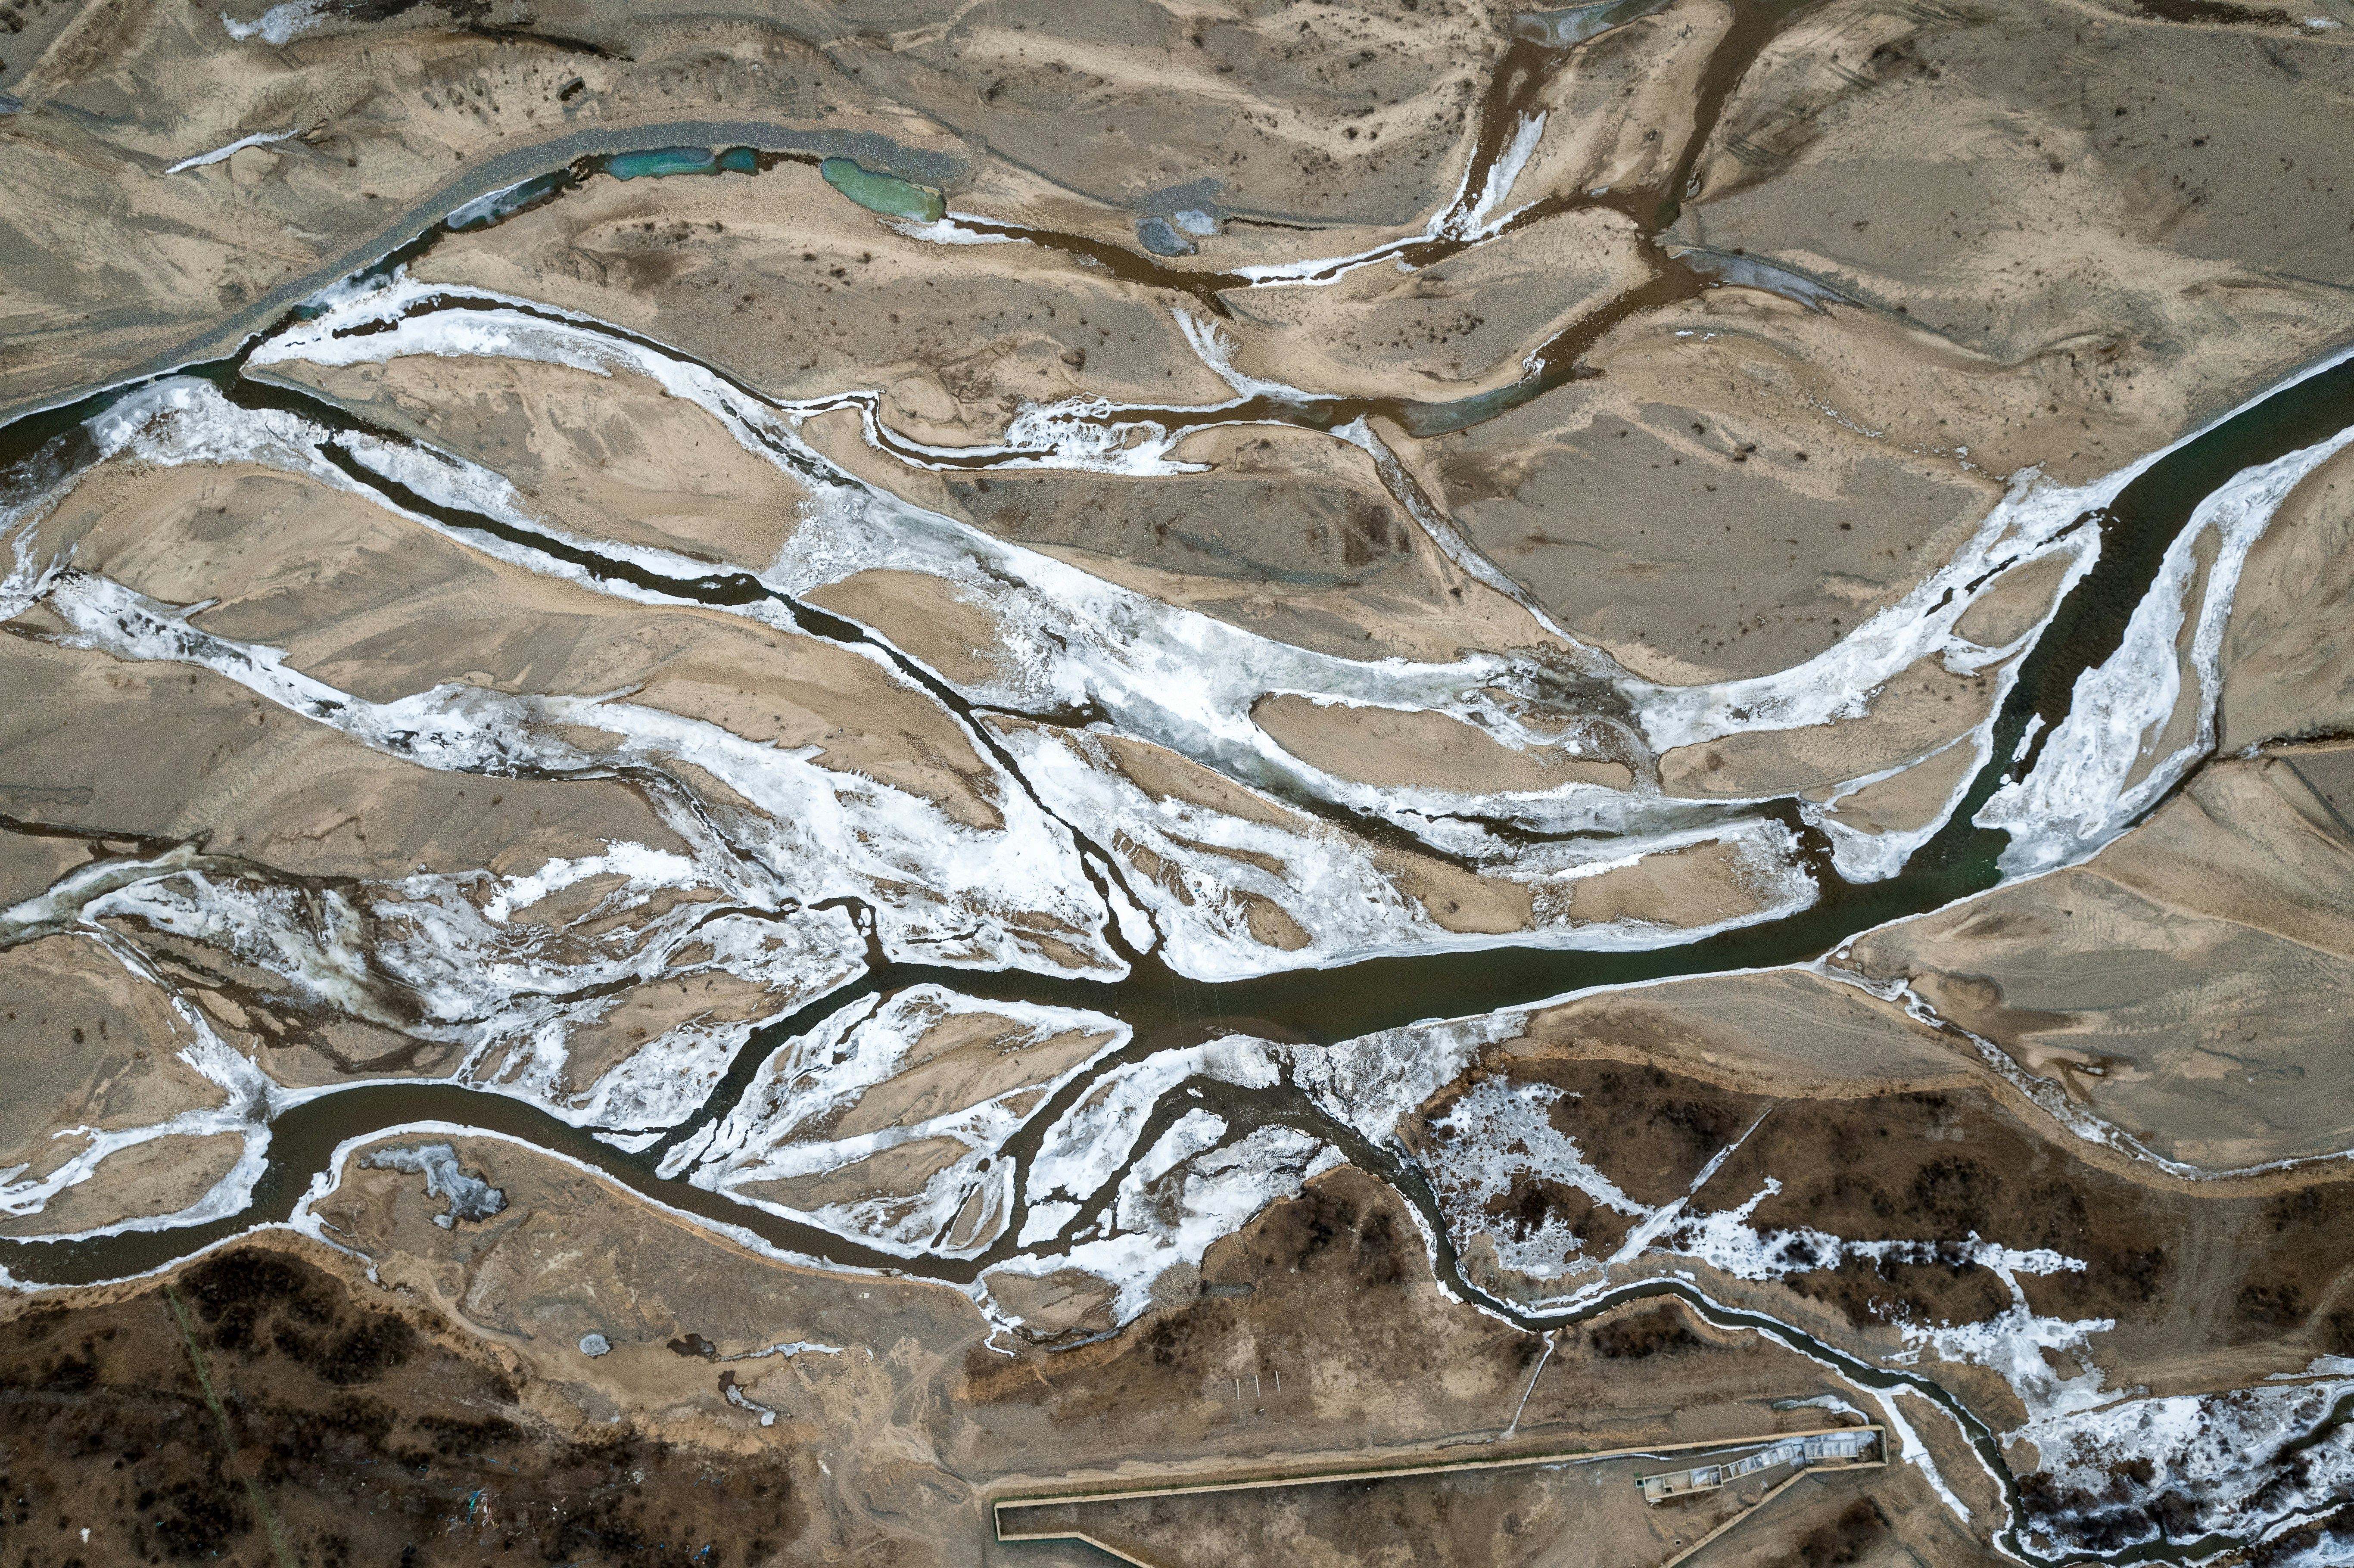
\includegraphics[width=\linewidth]{figures/rivers.jpg}
    \caption{Diffusive Waves}
  \end{subfigure}
\end{figure}
 \visible<1->{\begin{beamercolorbox}[rounded=true, shadow=true, wd=\textwidth]{block title}
 \centering Each can be formulated as a variational inequality with pointwise inequality constraints!
 \end{beamercolorbox}
 }
\end{frame}

%\begin{frame}[plain,c]
\begin{frame}{Discretization}
%\frametitle{A first slide}
\vfill
\visible<1->{
\Large When we solve PDEs (or VIs) on a computer, we choose an \textit{\alert{ansatz}} for $u$ that turns the continuous problem into a discrete one:
}
\visible<2->{
\[\text{
\Large $u(x) \approx \sum_{i=1}^n u_i \phi_i(x)$ where $u_i$ are numbers, $\phi_i$ ``nice'' functions.}
\]}
\end{frame}

%\begin{frame}[plain,c]
\begin{frame}{LVPP: A Unified Framework}
%\frametitle{A first slide}
\vfill
\visible<1->{\Large Finding an \textbf{unified framework} ensuring the \textbf{ansatz} always satisfies a given inequality constraint is the starting point for the \textbf{LaVa project} and the \alert{\textit{Latent Variable Proximal Point Method (LVPP)}.}\vfill

}
\visible<2->{
\begin{minipage}{0.55\linewidth}
 \large \textbf{LVPP} uses techniques from convex analysis and optimization that yield a unique computational framework for handling inequality constraints.
\end{minipage}
\begin{minipage}{0.4\linewidth}
\begin{figure}[h]
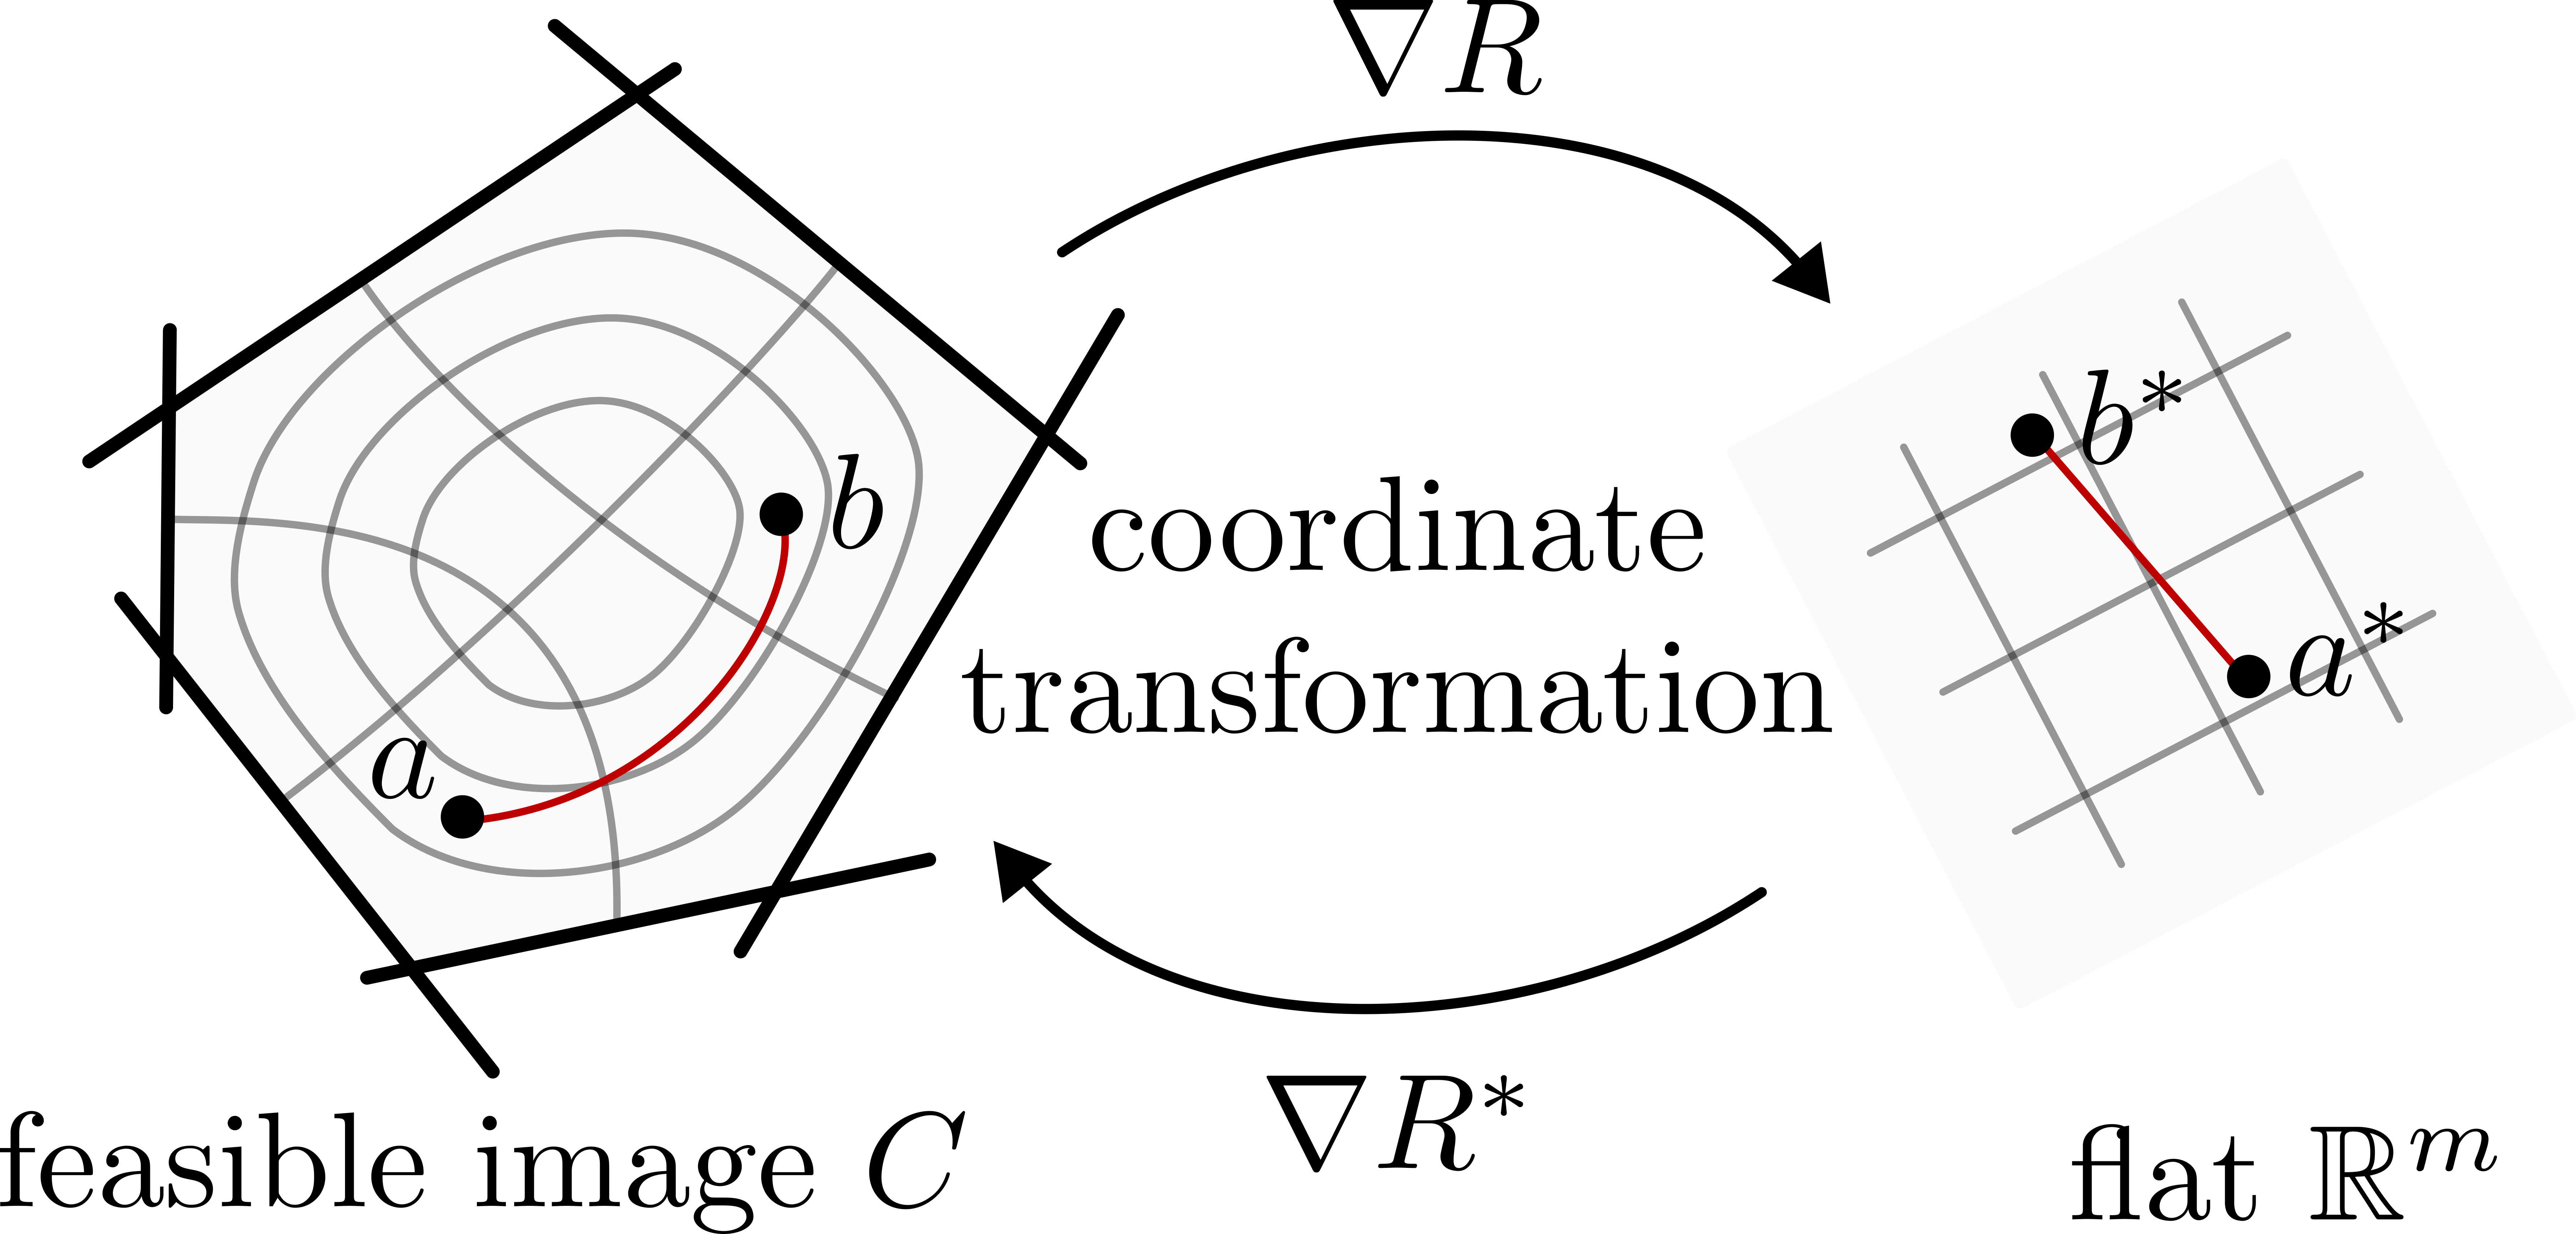
\includegraphics[width=0.8\linewidth]{figures/Geodesic3.png} 
\end{figure}
\end{minipage}
}
\vfill
\end{frame}



\end{document}